% -----------------------------------------------------------------------------
% DEXPI Beamer Theme
% -----------------------------------------------------------------------------
% Copyright (c) 2026 DEXPI e.V.
%
% This work is licensed under the Creative Commons Attribution-ShareAlike 4.0
% International License (CC BY-SA 4.0).
%
% You are free to:
%   - Share: copy and redistribute the material in any medium or format
%   - Adapt: remix, transform, and build upon the material for any purpose
%
% Under the following terms:
%   - Attribution: You must give appropriate credit to DEXPI e.V.,
%     provide a link to the license, and indicate if changes were made.
%   - ShareAlike: If you remix, transform, or build upon the material,
%     you must distribute your contributions under the same license.
%
% Full license text:
%   https://creativecommons.org/licenses/by-sa/4.0/
%
%  Author: Michael Wiedau
% -----------------------------------------------------------------------------

%----------------------------------------------------------------------------------------
%    PACKAGES AND THEMES
%----------------------------------------------------------------------------------------

\documentclass[aspectratio=169,xcolor=dvipsnames]{beamer}
\usetheme{DEXPI}

\usepackage{hyperref}
\usepackage{graphicx}
\usepackage{booktabs}
\usepackage{pgfgantt}
\usepackage[portuguese]{babel}


\usepackage{tikz}
\usepackage{circuitikz}
\usetikzlibrary{shapes.geometric,calc,positioning}
\usepackage{pgfplots}
\pgfplotsset{compat=1.10}
\usepackage{color}
\usepackage{listings}\usepackage{listings}
\usepackage{qrcode}


\newcommand{\hrefcol}[2]{\textcolor{cyan}{\href{#1}{#2}}}



% adicionar o numero na lista final da apresentação
\setbeamertemplate{bibliography item}{\insertbiblabel}


%----------------------------------------------------------------------------------------
%    TITLE PAGE
%----------------------------------------------------------------------------------------

\title{Autoencoders}
%\subtitle{Licensed under CC-BY-SA}
\author{Alice Cipriano \\ Leandro Fernandes}
\institute{CPE727 - Aprendizado Profundo}
\date{\today}

%----------------------------------------------------------------------------------------
%    PRESENTATION SLIDES
%----------------------------------------------------------------------------------------

\begin{document}
\begin{frame}[plain]
    \titlepage
\end{frame}

\begin{frame}{Sumário}
    % Throughout your presentation, if you choose to use \section{} and \subsection{} commands, these will automatically be printed on this slide as an overview of your presentation
    \tableofcontents
\end{frame}

%------------------------------------------------
\section{Introdução}

\begin{frame}{Objetivo}
    O objetivo principal deste trabalho é apresentar os conceitos teóricos de Autoencoders e representações esparsas, fundamentando-se no Capítulo 14 da literatura de referência \cite{Goodfellow2016}.
\end{frame}

\begin{frame}{O que é um Autoencoder?}
    \begin{itemize}
        \item Rede neural treinada para \textbf{copiar a entrada na saída}, passando por um \textbf{código} $h$ (representação latente);
        \item Duas partes: \textbf{encoder} $h = f(x)$ e \textbf{decoder} $r = g(h)$.
    \end{itemize}
    \vspace{-0.1cm}
    \centering
    \begin{tikzpicture}[scale=0.75, every node/.style={font=\small}]
        % encoder (trapézio que estreita)
        \fill[dexpiBlueLight] (0,-1.4) -- (2.6,-0.5) -- (2.6,0.5) -- (0,1.4) -- cycle;
        \draw[dexpiBlue, thick] (0,-1.4) -- (2.6,-0.5) -- (2.6,0.5) -- (0,1.4) -- cycle;
        \node[dexpiBlue] at (1.3,0) {\textbf{Encoder} $f$};
        % código
        \fill[dexpiGreenLight] (2.8,-0.5) rectangle (3.6,0.5);
        \draw[dexpiGreenDark, thick] (2.8,-0.5) rectangle (3.6,0.5);
        \node[dexpiGreenDark] at (3.2,0) {$h$};
        % decoder (trapézio que alarga)
        \fill[dexpiBlueLight] (3.8,-0.5) -- (6.4,-1.4) -- (6.4,1.4) -- (3.8,0.5) -- cycle;
        \draw[dexpiBlue, thick] (3.8,-0.5) -- (6.4,-1.4) -- (6.4,1.4) -- (3.8,0.5) -- cycle;
        \node[dexpiBlue] at (5.1,0) {\textbf{Decoder} $g$};
        % entrada e saída
        \node (x) at (-1.0,0) {\Large $x$};
        \node (r) at (7.4,0) {\Large $r$};
        \draw[->, thick] (x) -- (-0.05,0);
        \draw[->, thick] (6.45,0) -- (r);
        \node[below, align=center, font=\scriptsize] at (3.2,-1.5) {código (representação latente)};
    \end{tikzpicture}
 
    \vspace{-0.1cm}
    \begin{alertblock}{Paradoxo}
        Se aprender $g(f(x)) = x$ perfeitamente, é inútil. O autoencoder é \textbf{projetado para não conseguir copiar perfeitamente}: precisa escolher o que guardar.
    \end{alertblock}
\end{frame}

\begin{frame}{Exemplo concreto: dígitos manuscritos}
    \begin{columns}[c, onlytextwidth]
        \begin{column}{0.42\textwidth}
            \small
            \begin{itemize}
                \item Imagens $8 \times 8$ $\rightarrow$ $x \in \mathbb{R}^{64}$;
                \item Código $h \in \mathbb{R}^{8}$: \textbf{8$\times$ menor};
                \item MLP denso: $64 \rightarrow 32 \rightarrow \textbf{8} \rightarrow 32 \rightarrow 64$;
                \item ReLU, treinado com Adam e MSE;
                \item Alvo do treino = a própria entrada.
            \end{itemize}
            \vspace{0.1cm}
            \begin{exampleblock}{Importante}
                Reconstrução \textbf{aproximada}: guarda o formato, descarta detalhes.
            \end{exampleblock}
        \end{column}
        \begin{column}{0.56\textwidth}
            \centering
            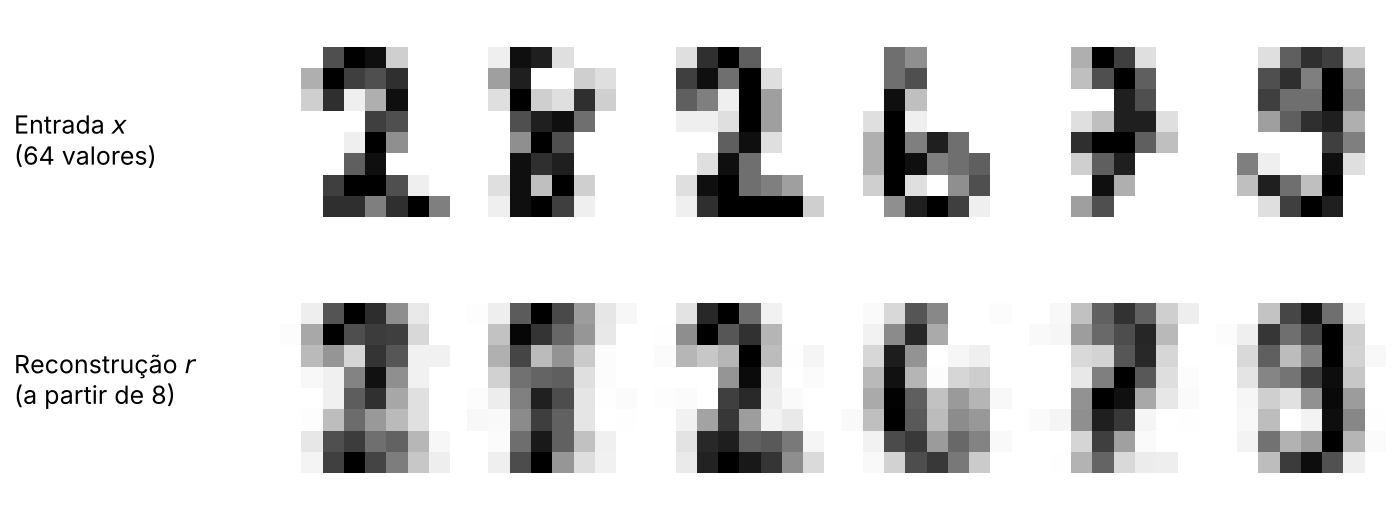
\includegraphics[width=1\textwidth]{figures/Alice/ae_digitos_reconstrucao.png}\\
            {\scriptsize Autoencoder treinado no \textit{digits} (scikit-learn), conjunto de teste.}
        \end{column}
    \end{columns}
\end{frame}
 
\begin{frame}{Autoencoders: visão geral}
    \begin{block}{Do determinístico ao estocástico}
        \begin{itemize}
            \item Clássico: funções $f(x)$ e $g(h)$;
            \item Moderno: distribuições $p_{\text{encoder}}(h \mid x)$ e $p_{\text{decoder}}(x \mid h)$ $\rightarrow$ base dos modelos generativos (VAE).
        \end{itemize}
    \end{block}
    \begin{itemize}
        \item \textbf{Usos tradicionais:} redução de dimensionalidade e aprendizado de \textit{features};
        \item \textbf{Usos recentes:} modelagem generativa, via conexão com modelos de variáveis latentes;
        \item \textbf{Treinamento:} caso especial de rede \textit{feedforward} $\rightarrow$ gradiente descendente em minibatch + \textit{backpropagation};
        \item Alternativa histórica: \textbf{recirculação} (Hinton \& McClelland, 1988), mais plausível biologicamente, pouco usada.
    \end{itemize}
\end{frame}

%------------------------------------------------
\section{Autoencoders Incompletos e Regularizados}

\begin{frame}{Autoencoders Incompletos (\textit{Undercomplete})}
    \begin{itemize}
        \item Em geral, não interessa a saída do decoder, e sim as propriedades que $h$ aprende;
        \item Restrição mais simples: \textbf{gargalo}, $\dim(h) < \dim(x)$ $\rightarrow$ captura as características mais salientes dos dados;
        \item Treinamento: minimizar uma função de perda
    \end{itemize}
    \[
        L\big(x,\; g(f(x))\big)
        \qquad \text{ex.: } \; L = \lVert x - g(f(x)) \rVert^2 \;\; \text{(MSE)}
    \]
    \begin{block}{Outras perdas comuns}
        \begin{itemize}
            \item Dados binários ou em $[0,1]$: entropia cruzada binária;
            \item Dados com \textit{outliers}: erro absoluto (MAE);
            \item Dados categóricos: entropia cruzada com softmax.
        \end{itemize}
    \end{block}
\end{frame}
 
\begin{frame}{Relação com PCA}
    \begin{itemize}
        \item Decoder \textbf{linear} + MSE $\rightarrow$ aprende o \textbf{mesmo subespaço do PCA};
        \item $f$ e $g$ \textbf{não lineares} (ativações como $\tanh$ entre as camadas) $\rightarrow$ generalização não linear do PCA: captura estruturas curvas.
    \end{itemize}
    \centering
    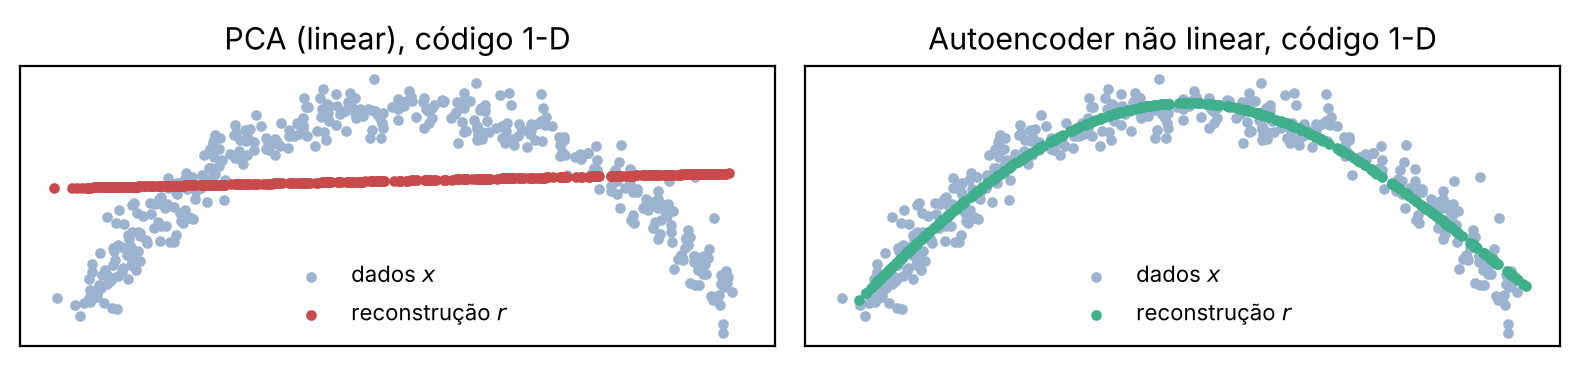
\includegraphics[width=0.78\textwidth]{figures/Alice/pca_vs_ae.png}\\
    {\scriptsize Dados 2-D sobre um arco, comprimidos para 1 dimensão. Autoencoder: $2 \rightarrow 32 \rightarrow 1 \rightarrow 32 \rightarrow 2$ com $\tanh$.\\ MSE: PCA $\approx 0{,}015$; autoencoder $\approx 0{,}001$.}
\end{frame}
 
\begin{frame}{O risco: capacidade demais}
    \begin{itemize}
        \item Encoder e decoder poderosos demais copiam \textbf{sem aprender} a distribuição dos dados;
        \item O gargalo sozinho não garante nada.
    \end{itemize}
    \begin{alertblock}{Exemplo extremo (teórico)}
        \begin{itemize}
            \item Código de \textbf{uma única dimensão};
            \item Encoder mapeia o $i$-ésimo exemplo $x^{(i)}$ para o número $i$;
            \item Decoder aprende a tabela $i \mapsto x^{(i)}$.
        \end{itemize}
        Reconstrução perfeita no treino, mas $h$ é só um índice: o modelo \textbf{memorizou} os exemplos (\textit{overfitting}).
    \end{alertblock}
\end{frame}
 
\begin{frame}{Autoencoders Regularizados}
    \begin{itemize}
        \item $\dim(h) = \dim(x)$ ou $\dim(h) > \dim(x)$ (\textbf{overcomplete}): até encoder e decoder lineares copiam perfeitamente;
        \item Ideia: em vez de limitar a arquitetura, \textbf{mudar a função de perda} para exigir outras propriedades além de copiar.
    \end{itemize}
    \vspace{0.1cm}
    \centering
    \small
    \begin{tabular}{@{}lll@{}}
        \toprule
        \textbf{Propriedade exigida} & \textbf{Modelo} & \textbf{Perda} \\
        \midrule
        Representação esparsa & Sparse AE & $L(x, g(f(x))) + \Omega(h)$ \\
        Robustez a ruído & Denoising AE & $L(x, g(f(\tilde{x})))$ \\
        Derivada pequena & Contractive AE & $L(x, g(f(x))) + \Omega(h, x)$ \\
        \bottomrule
    \end{tabular}
    \vspace{0.2cm}
    \begin{block}{Resultado}
        Modelos grandes, não lineares e até \textit{overcomplete} que ainda aprendem algo útil sobre os dados.
    \end{block}
\end{frame}
 
\begin{frame}{Sparse Autoencoders}
    \begin{itemize}
        \item Adiciona uma penalidade de esparsidade $\Omega(h)$ sobre o código:
    \end{itemize}
    \[
        L\big(x,\, g(f(x))\big) + \Omega(h), \qquad \Omega(h) = \lambda \sum_i |h_i| \;\; \text{(norma L1)}
    \]
    \begin{itemize}
        \item \textbf{Esparso:} a maioria das unidades de $h$ é zero para cada exemplo;
    \end{itemize}
    \centering
    \begin{tikzpicture}[cell/.style={draw=dexpiBlue, minimum width=0.8cm, minimum height=0.5cm, font=\scriptsize}]
        \node[anchor=east, font=\small] at (0.3,0) {Denso:};
        \foreach \v [count=\i] in {0.3,-0.7,0.2,0.9,-0.1,0.4,0.6,-0.5}
            \node[cell, fill=dexpiBlueLight] at (0.8*\i,0) {\v};
        \node[anchor=east, font=\small] at (0.3,-0.7) {Esparso:};
        \foreach \v [count=\i] in {0,0,1.2,0,0,0,0.8,0}
            \node[cell, fill=white] at (0.8*\i,-0.7) {\v};
        \node[cell, fill=dexpiGreenLight] at (0.8*3,-0.7) {1.2};
        \node[cell, fill=dexpiGreenLight] at (0.8*7,-0.7) {0.8};
    \end{tikzpicture}
    \begin{itemize}
        \item Reconstrução pede usar $h$; $\Omega$ pede usar $h$ o mínimo possível $\rightarrow$ só o essencial é guardado;
        \item Uso típico: \textit{features} para outra tarefa (ex.: classificação).
    \end{itemize}
\end{frame}
 
\begin{frame}{Sparse Autoencoders: visão probabilística}
    \begin{itemize}
        \item Modelo com visíveis $x$ e latentes $h$: $\;p_{\text{model}}(x, h) = p_{\text{model}}(h)\, p_{\text{model}}(x \mid h)$;
        \item $\log p(x) = \log \sum_h p(h, x)$ em geral é intratável $\rightarrow$ o autoencoder usa \textbf{um único} $h = f(x)$:
    \end{itemize}
    \[
        \log p_{\text{model}}(h, x) = \underbrace{\log p_{\text{model}}(h)}_{\text{a priori sobre } h} + \underbrace{\log p_{\text{model}}(x \mid h)}_{\text{reconstrução}}
    \]
    \begin{block}{Distribuição a priori de Laplace $\rightarrow$ penalidade L1}
        \[
            p(h_i) = \frac{\lambda}{2} e^{-\lambda |h_i|}
            \;\;\Rightarrow\;\;
            -\log p(h) = \sum_i \Big(\lambda |h_i| - \log \tfrac{\lambda}{2}\Big) = \Omega(h) + \text{const}
        \]
    \end{block}
    \begin{itemize}
        \item A esparsidade não é um regularizador arbitrário: é \textbf{consequência} de acreditar que os latentes costumam ser zero.
    \end{itemize}
\end{frame}
 
\begin{frame}{Sparse Autoencoders: observações}
    \begin{block}{Comparação: weight decay (regularizador usual) $\times$ esparsidade}
        \begin{itemize}
            \item \textbf{Weight decay} $\lambda \lVert \theta \rVert^2$: a priori sobre os \textbf{pesos} $\theta$, escolhida antes de ver os dados (MAP);
            \item \textbf{Esparsidade} $\Omega(h)$: depende de $h = f(x)$, ou seja, \textbf{muda com cada entrada}. É a priori sobre os \textbf{latentes} $h$, não sobre $\theta$.
        \end{itemize}
    \end{block}
    \begin{itemize}
        \item \textbf{Ativação do código:} a L1 já induz esparsidade com qualquer ativação, mas com sigmoide ou $\tanh$ os valores ficam só \textit{perto} de zero. Com ReLU, $\max(0, z)$, toda ativação negativa vira \textbf{exatamente} 0 (Glorot et al., 2011).
    \end{itemize}
\end{frame}


%------------------------------------------------
\section{Capacidade de Representação, Camadas e Profundidades}

\begin{frame}{Por que autoencoders profundos?}
    \small
    \begin{itemize}
        \item Encoder e decoder são, cada um, uma rede \textit{feedforward} $\rightarrow$ \textbf{cada parte} se beneficia de profundidade.
    \end{itemize}
    \begin{block}{O argumento do teorema da aproximação universal}
        \begin{itemize}
            \item Uma rede com $\geq 1$ camada oculta aproxima qualquer função, com unidades suficientes;
            \item \textbf{Raso:} o mapeamento $x \rightarrow h$ é uma camada só $\rightarrow$ não dá para impor restrições arbitrárias ao código (ex.: ser esparso);
            \item \textbf{Profundo:} com $\geq 1$ camada oculta \textbf{dentro do encoder}, ele aproxima qualquer mapeamento $x \rightarrow h$.
        \end{itemize}
    \end{block}
    \begin{itemize}
        \item A profundidade pode reduzir \textbf{exponencialmente} o custo computacional e a quantidade de dados necessária para algumas funções.
    \end{itemize}
\end{frame}
 
\begin{frame}{Profundidade na prática}
    \begin{columns}[c, onlytextwidth]
        \begin{column}{0.38\textwidth}
            \small
            \begin{itemize}
                \item Dígitos $8 \times 8$, mesmo código $h$ de \textbf{8} dimensões;
                \item Muda só o número de camadas ($\tanh$).
            \end{itemize}
            \begin{exampleblock}{Leitura do gráfico}
                Raso $\approx$ PCA. Cada camada a mais reduz o erro: o mais profundo erra cerca de \textbf{metade} do PCA.
            \end{exampleblock}
            {\scriptsize Resultado alinhado com Hinton \& Salakhutdinov (2006).}
        \end{column}
        \begin{column}{0.60\textwidth}
            \centering
            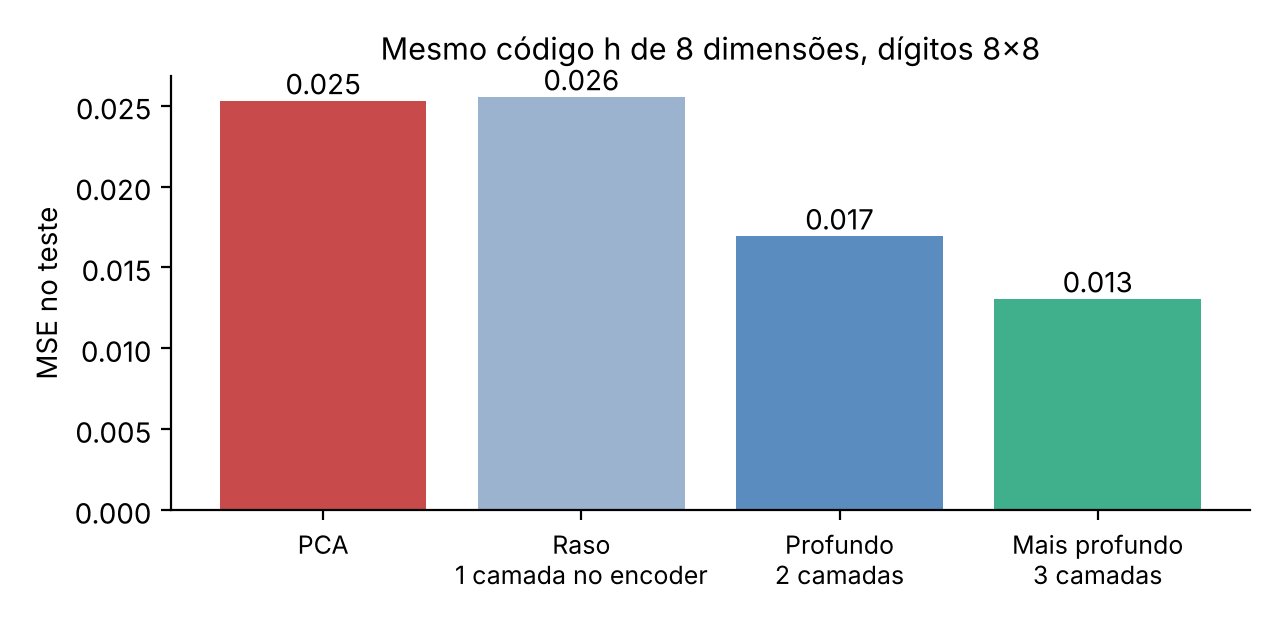
\includegraphics[width=1\textwidth]{figures/Alice/raso_vs_profundo.png}\\
            {\scriptsize MSE no conjunto de teste, média de 3 inicializações.}
        \end{column}
    \end{columns}
\end{frame}
 
\begin{frame}{Pré-treino guloso em camadas}
    \begin{itemize}
        \item Estratégia comum para treinar autoencoders profundos: \textbf{empilhar autoencoders rasos}, treinados um de cada vez.
    \end{itemize}
    \centering
    \begin{tikzpicture}[scale=0.85, transform shape,
        lay/.style={draw=dexpiBlue, fill=dexpiBlueLight, rounded corners=2pt, minimum width=0.9cm, minimum height=0.55cm, font=\small},
        cod/.style={draw=dexpiGreenDark, fill=dexpiGreenLight, rounded corners=2pt, minimum width=0.9cm, minimum height=0.55cm, font=\small},
        stp/.style={font=\scriptsize\bfseries, text=dexpiBlue}, >=stealth]
        % passo 1
        \node[stp] at (1.2,1.0) {1. Treina AE raso};
        \node[lay] (a1) at (0,0) {$x$}; \node[cod] (a2) at (1.2,0) {$h_1$}; \node[lay] (a3) at (2.4,0) {$\hat{x}$};
        \draw[->] (a1) -- (a2); \draw[->] (a2) -- (a3);
        % passo 2
        \node[stp] at (5.4,1.0) {2. Treina AE sobre $h_1$};
        \node[lay] (b1) at (4.2,0) {$h_1$}; \node[cod] (b2) at (5.4,0) {$h_2$}; \node[lay] (b3) at (6.6,0) {$\hat{h}_1$};
        \draw[->] (b1) -- (b2); \draw[->] (b2) -- (b3);
        % passo 3
        \node[stp] at (10.4,1.0) {3. Empilha e ajusta};
        \node[lay] (c1) at (8.2,0) {$x$}; \node[lay] (c2) at (9.3,0) {$h_1$}; \node[cod] (c3) at (10.4,0) {$h_2$};
        \node[lay] (c4) at (11.5,0) {$\hat{h}_1$}; \node[lay] (c5) at (12.6,0) {$\hat{x}$};
        \draw[->] (c1) -- (c2); \draw[->] (c2) -- (c3); \draw[->] (c3) -- (c4); \draw[->] (c4) -- (c5);
        \draw[dexpiBlue, dashed] (3.3,-0.6) -- (3.3,1.2); \draw[dexpiBlue, dashed] (7.5,-0.6) -- (7.5,1.2);
    \end{tikzpicture}
    \begin{itemize}
        \item \textbf{Guloso:} cada camada é otimizada sozinha, sem considerar as seguintes;
        \item Depois de empilhar, a rede inteira é ajustada com \textit{backpropagation} (\textit{fine-tuning}).
    \end{itemize}
    \begin{exampleblock}{Contexto histórico}
        Usado quando o gradiente ``sumia'' em redes profundas. Hoje (ReLU, boas inicializações) treina-se direto; a ideia reaparece no CAE.
    \end{exampleblock}
\end{frame}


%------------------------------------------------
\section{Autoencoders Estocásticos}

\begin{frame}{A perda vem de uma distribuição}
    \begin{itemize}
        \item Receita geral das redes \textit{feedforward}: definir $p(y \mid x)$ e minimizar $-\log p(y \mid x)$;
        \item No autoencoder, $x$ é \textbf{entrada e alvo}: o decoder define $p_{\text{decoder}}(x \mid h)$ e minimizamos
    \end{itemize}
    \[
        -\log p_{\text{decoder}}(x \mid h)
    \]
    \centering
    \small
    \begin{tabular}{@{}llll@{}}
        \toprule
        \textbf{Tipo de $x$} & \textbf{Escolha usual de $p_{\text{decoder}}$} & \textbf{Unidade de saída} & \textbf{$-\log p_{\text{decoder}}$ vira} \\
        \midrule
        Real & Gaussiana (média $= g(h)$) & Linear & MSE \\
        Binário & Bernoulli & Sigmoide & Entropia cruzada binária \\
        Discreto & Softmax (categórica) & Softmax & Entropia cruzada \\
        \bottomrule
    \end{tabular}
    \vspace{0.2cm}
    \begin{block}{Por que isso importa}
        Escolher a perda $=$ escolher a distribuição do decoder. Ex.: gaussiana com variância fixa $\Rightarrow -\log p = \frac{1}{2\sigma^2}\lVert x - g(h) \rVert^2 + \text{const}$, ou seja, MSE.
    \end{block}
\end{frame}
 
\begin{frame}{Encoder e decoder estocásticos}
    \begin{itemize}
        \item Generalização: a \textbf{função} $f(x)$ vira uma \textbf{distribuição} $p_{\text{encoder}}(h \mid x)$, e $g(h)$ vira $p_{\text{decoder}}(x \mid h)$;
        \item A saída de cada parte é \textbf{sorteada}: há injeção de ruído.
    \end{itemize}
    \centering
    \begin{tikzpicture}[scale=0.85, transform shape,
        box/.style={draw=dexpiBlue, fill=dexpiBlueLight, rounded corners=2pt, minimum height=0.7cm, font=\small, align=center},
        cod/.style={draw=dexpiGreenDark, fill=dexpiGreenLight, rounded corners=2pt, minimum height=0.7cm, minimum width=0.8cm, font=\small},
        >=stealth]
        \node (x) at (0,0) {\Large $x$};
        \node[box] (enc) at (2.6,0) {Encoder\\$p_{\text{encoder}}(h \mid x)$};
        \node[cod] (h) at (5.3,0) {$h$};
        \node[box] (dec) at (8.0,0) {Decoder\\$p_{\text{decoder}}(x \mid h)$};
        \node (r) at (10.6,0) {\Large $r$};
        \draw[->, thick] (x) -- (enc); \draw[->, thick] (enc) -- (h); \draw[->, thick] (h) -- (dec); \draw[->, thick] (dec) -- (r);
        \node[font=\scriptsize, text=dexpiGreenDark] at (5.3,-0.6) {sorteado};
    \end{tikzpicture}
 
    {\scriptsize Estrutura de um autoencoder estocástico.}
    \vspace{0.2cm}
    \begin{itemize}
        \item Em geral, supõe-se que as componentes de $x$ são \textbf{independentes dado $h$}: $p(x \mid h) = \prod_j p(x_j \mid h)$ $\rightarrow$ perda barata (soma termo a termo).
    \end{itemize}
\end{frame}
 
\begin{frame}{Ligação com modelos de variáveis latentes}
    \begin{itemize}
        \item Um modelo $p_{\text{model}}(h, x)$ trata código e dado como variáveis aleatórias ($x$ observado, $h$ escondido);
        \item Ele define naturalmente um encoder e um decoder estocásticos:
    \end{itemize}
    \[
        \underbrace{p_{\text{encoder}}(h \mid x) = p_{\text{model}}(h \mid x)}_{\text{inferência: dado } x\text{, quais } h \text{ são prováveis?}}
        \qquad\quad
        \underbrace{p_{\text{decoder}}(x \mid h) = p_{\text{model}}(x \mid h)}_{\text{geração: dado } h\text{, quais } x \text{ são prováveis?}}
    \]
    \vspace{0.2cm}
    \begin{alertblock}{Problema: compatibilidade}
        Treinados separadamente, encoder e decoder podem não vir da \textbf{mesma} distribuição conjunta. Treinar como \textbf{denoising autoencoder} tende a torná-los compatíveis.
    \end{alertblock}
\end{frame}



%------------------------------------------------
\section{Manifolds com Autoencoders}

\begin{frame}{Manifolds com Autoencoders}

O que são Manifolds? Conceito apresentado em 5.11.3.
\begin{columns}[c, onlytextwidth]
    \begin{column}{0.33\textwidth}
        \centering
        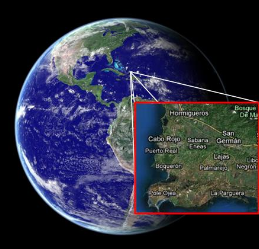
\includegraphics[width=1\textwidth]{figures/Fernandes/manifold_example.png}
        % \bibitem{campana2011} R. Campana-Olivo and V. Manian, ``Parallel implementation of nonlinear dimensionality reduction methods applied in object segmentation using CUDA in GPU,'' in \emph{Proc. SPIE}, vol. 8048, 2011.
    \end{column}
    
    \begin{column}{0.33\textwidth}
        \centering
        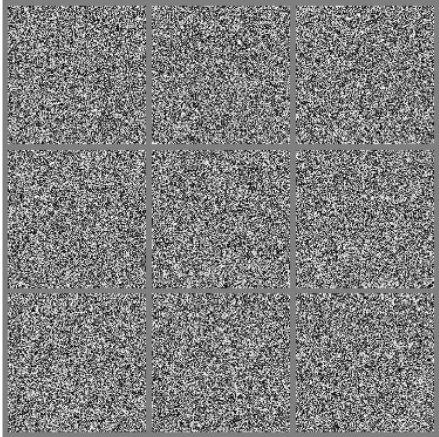
\includegraphics[width=0.97\textwidth]{figures/Fernandes/aleatory_pixels.png}
    \end{column}
    
    \begin{column}{0.33\textwidth}
    \centering
    \scriptsize
    \textbf{Semelhança entre um\\ ser humano e...}
    
    \vspace{0.3cm}
    
    \begin{tabular}{@{}l r@{}}
        outro humano & $\sim$99,9\% \\
        Chimpanzés & $\sim$98,8\% \\
        Bonobos & $\sim$98,7\% \\
        Gorilas & $\sim$98,4\% \\
        Orangotangos & $\sim$97\% \\
        Gibões & $\sim$95\% \\
        Macacos Rhesus & $\sim$93\% \\
        Gatos (Abissínios) & $\sim$90\% \\
        Ratos & $\sim$85\% \\
        Cães & $\sim$84\% \\
        Vacas / Porcos & $\sim$80\% \\
    \end{tabular}
\end{column}

\end{columns}

\end{frame}

\begin{frame}{Manifolds com Autoencoders}

    \begin{itemize}
        \item Dados que fazem sentido se concentram em espaços de menores dimensões;
        \item Aprendizado de Máquina utilizam funções que se comportam bem com dados dentro desses espaços, apresentando comportamento anômalo para dados externos;  
    \end{itemize}
    \centering
    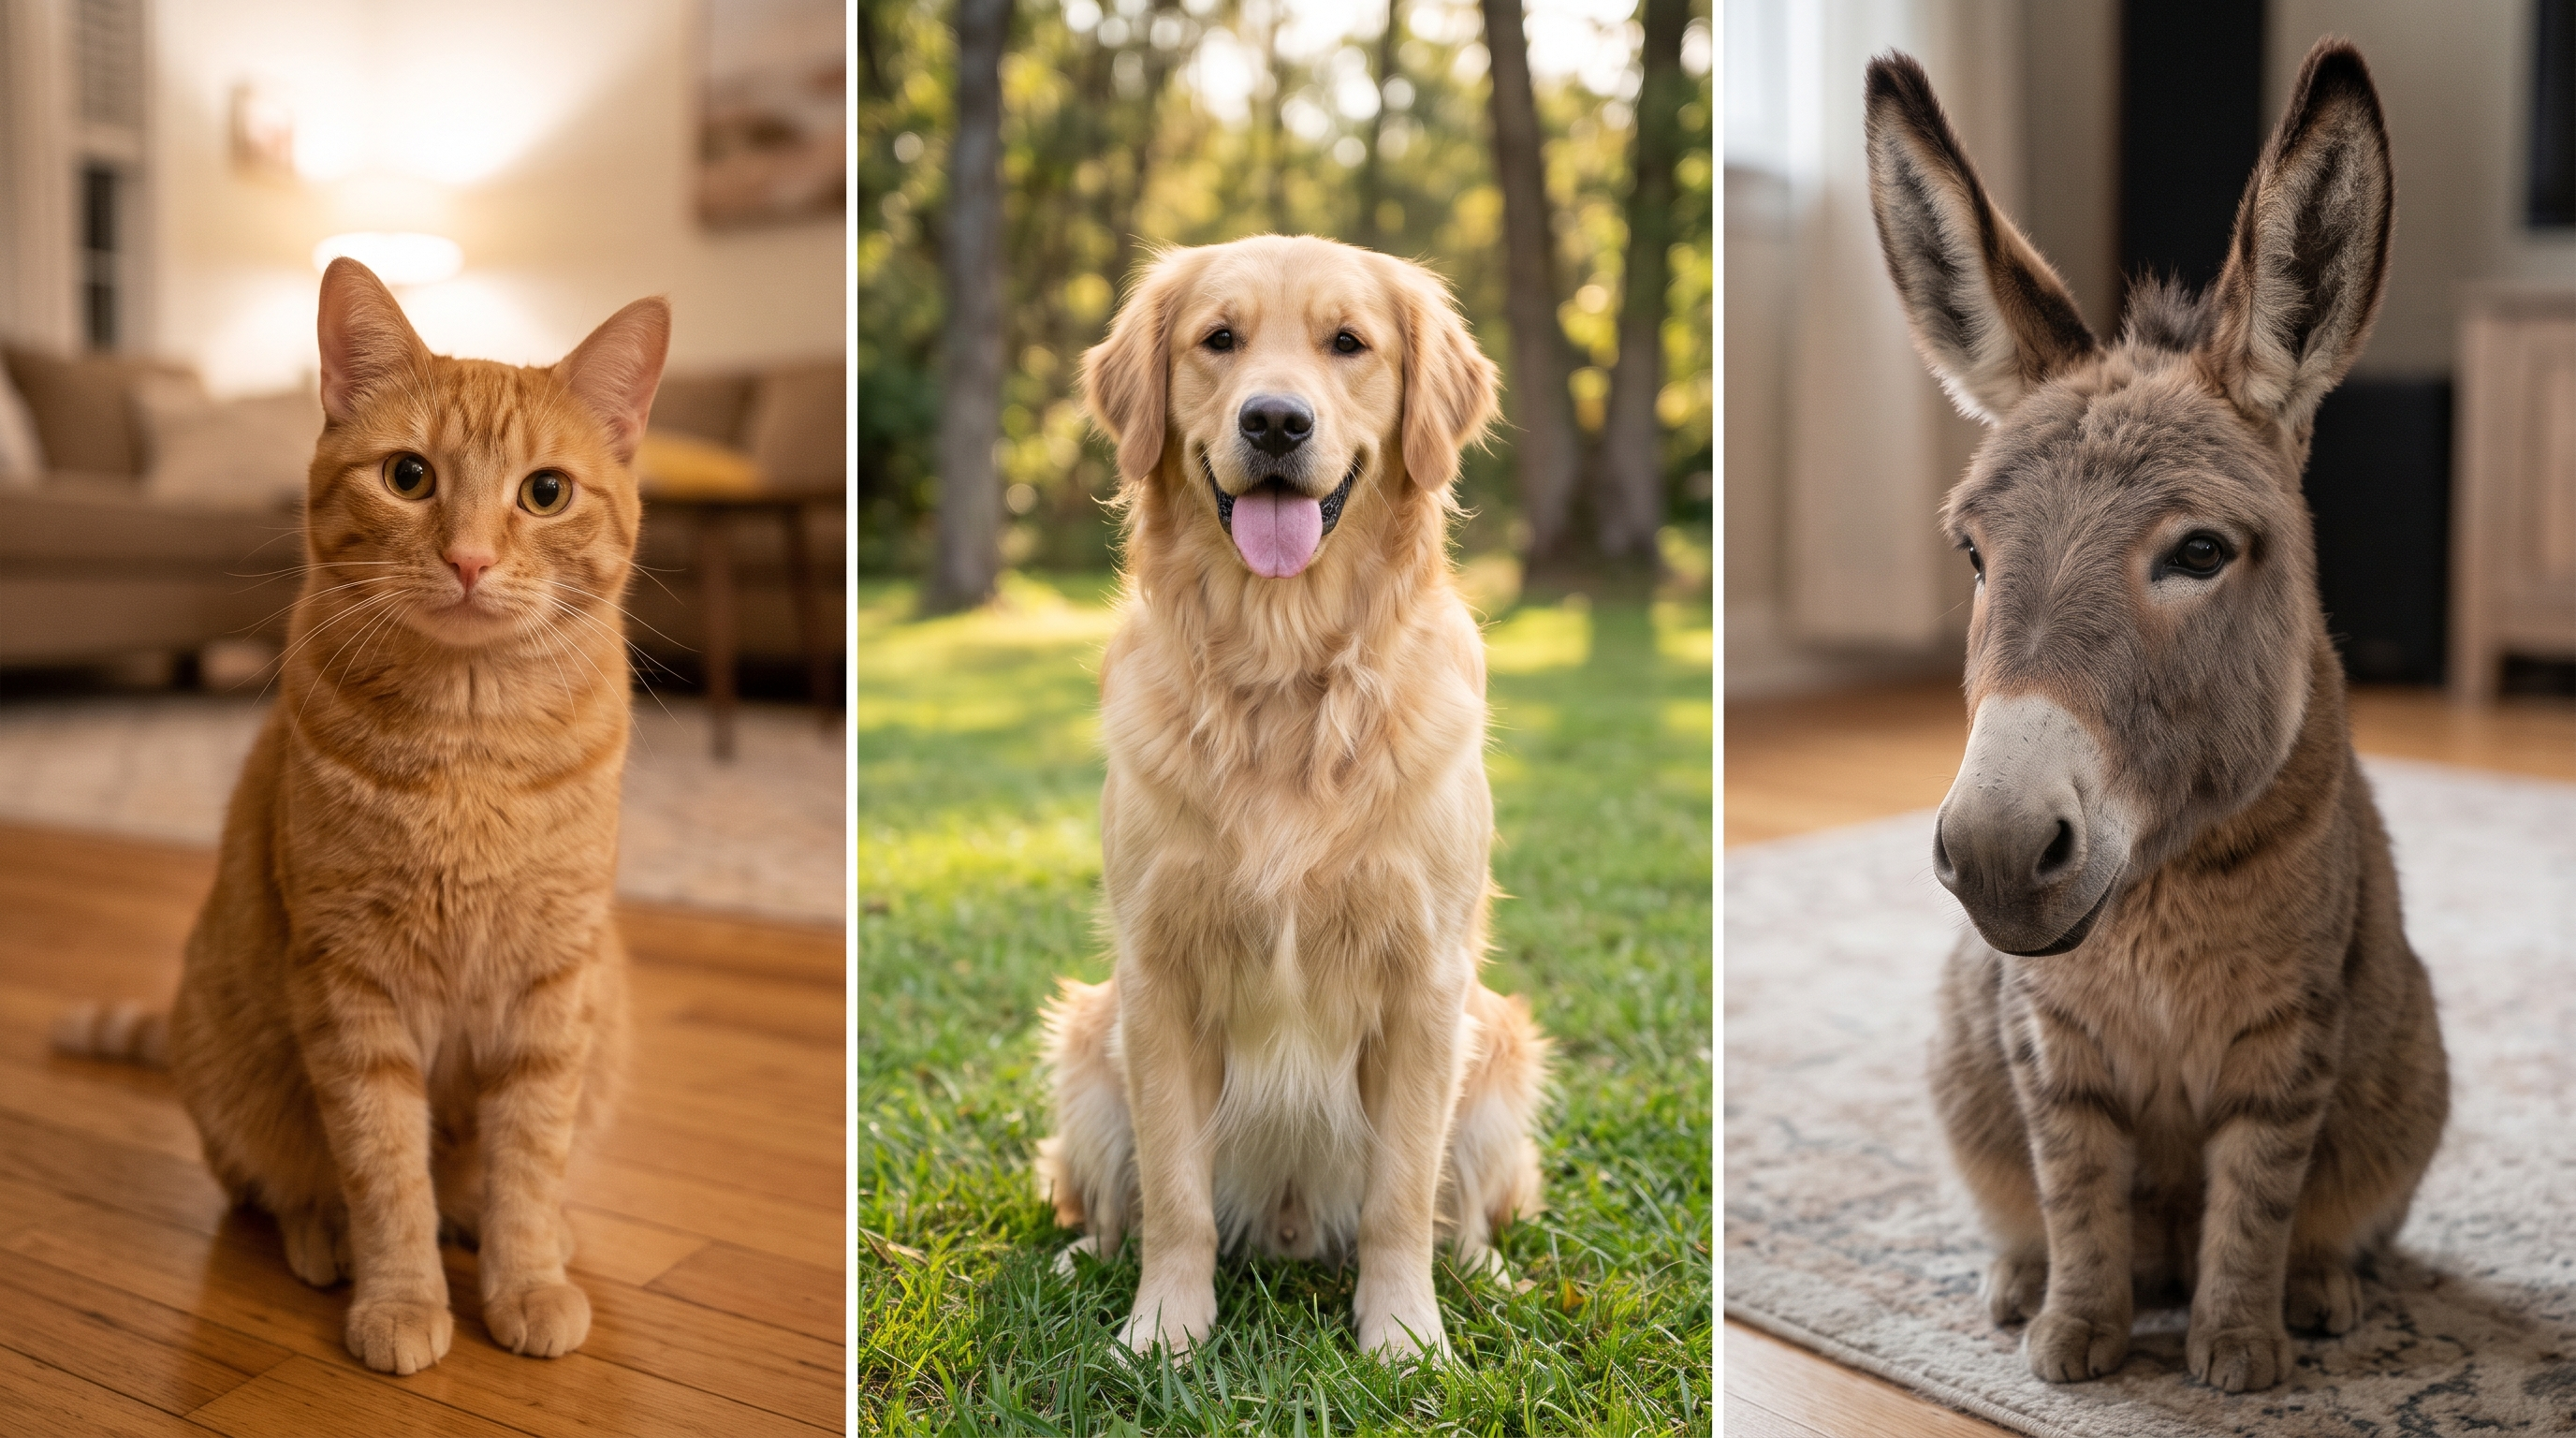
\includegraphics[width=0.50\textwidth]{figures/Fernandes/Dados_fora_do_Manifold.jpg}

\end{frame}


\begin{frame}{Manifolds com Autoencoders}
    \begin{block}{Treinamento de Autoencoders}
    Todo o treinamento de Autoencoders envolve uma solução de compromisso entre estes dois fatores:
    \begin{itemize}
        \item Aprender a representação do espaço latente $h$, de forma que $x$ possa ser aproximadamente recuperado: $\hat{x} = g(f(x)) \approx x$
        \item Satisfazer as restrições / regularizações aplicadas, adotando soluções pouco sensíveis aos dados de entrada.
    \end{itemize}
    \end{block}

    Estas duas forças devem atuar em conjunto, para forçar que a \textbf{camada oculta - h} capture informações importantes sobre a distribuição dos dados. Sendo assim, somente as variações úteis para a reconstrução dos dados serão obtidas.

\end{frame}

\begin{frame}{Manifolds com Autoencoders}
    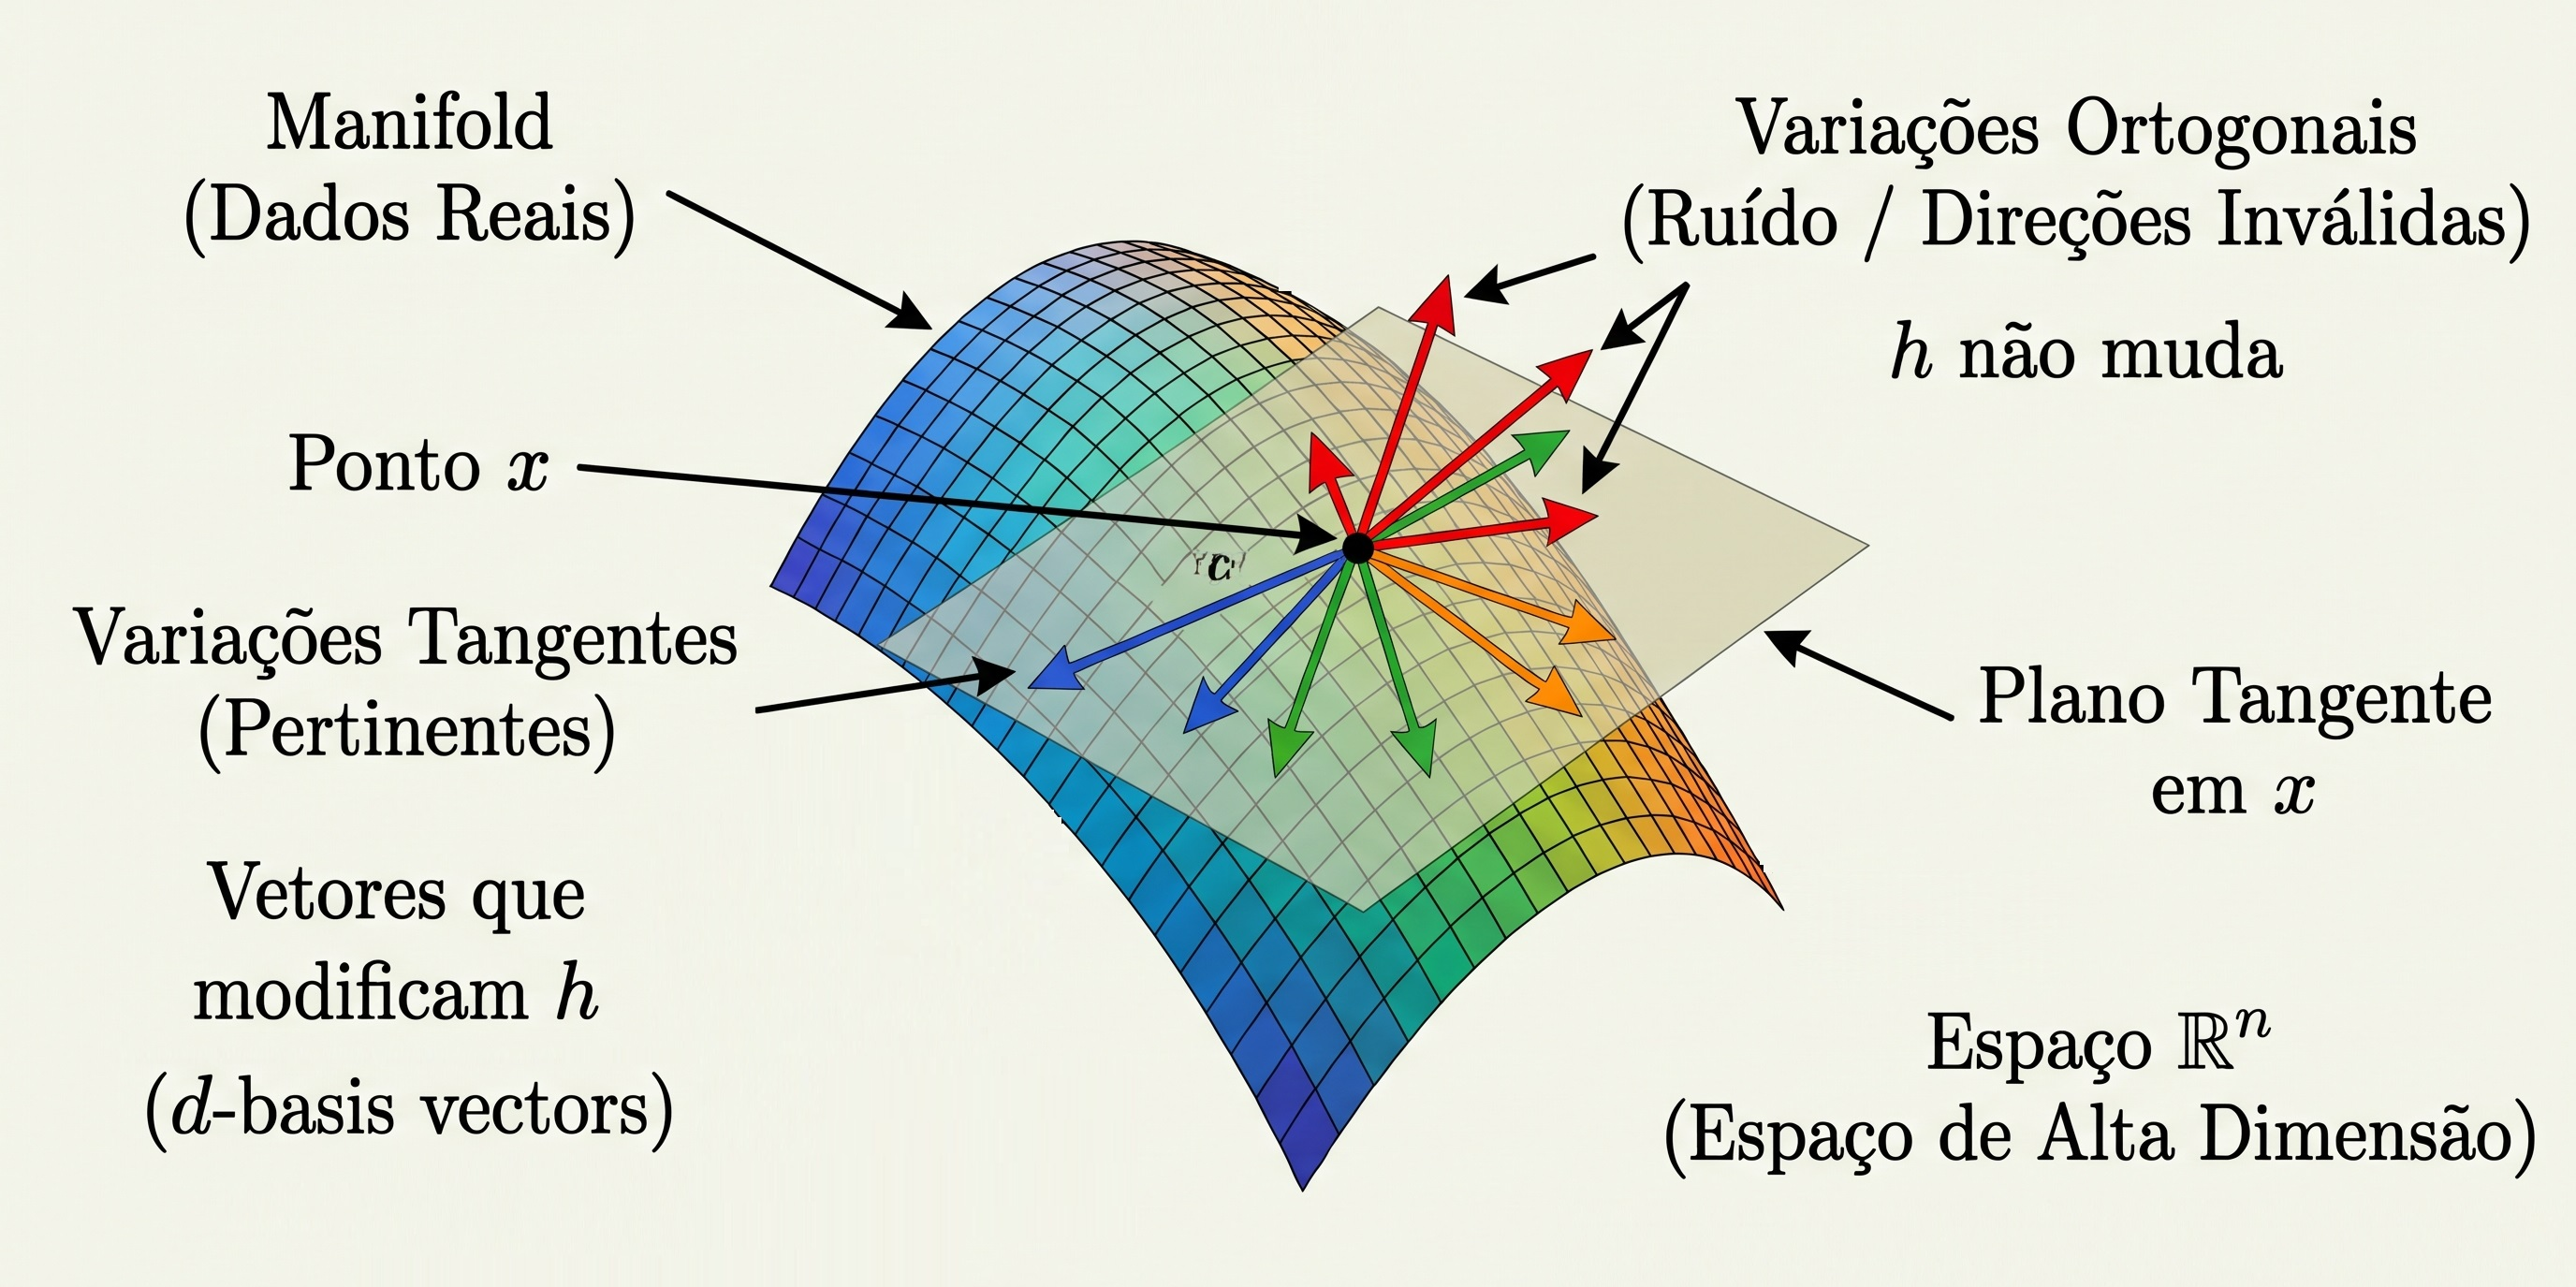
\includegraphics[width=0.95\textwidth]{figures/Fernandes/d_dimensional_manifold.jpg}
\end{frame}

\begin{frame}{Manifolds com Autoencoders}
    \centering
    Método não paramétrico - nearest-neighbor graph
    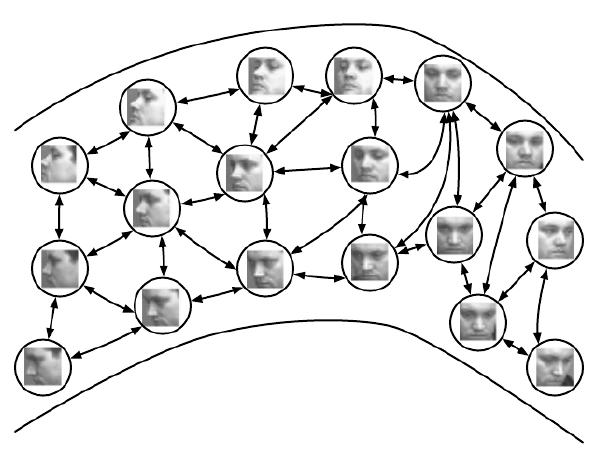
\includegraphics[width=0.6\textwidth]{figures/Fernandes/nearest-neighbor_graph.png}
\end{frame}
    
%------------------------------------------------
\section{Denoising Autoencoders}

\begin{frame}{Denoising Autoencoders}
    Projetado com uma degradação intencional nos dados de entrada de forma que consiga estimar dados de saída livres de ruídos.
    \begin{columns}
        \begin{column}{0.3\textwidth}
            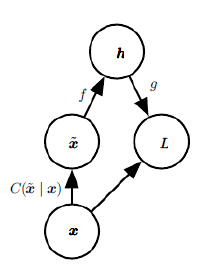
\includegraphics[width=0.95\textwidth]{figures/Fernandes/DAE_esquema.png}
        \end{column}

        \begin{column}{0.7\textwidth}
            \begin{itemize}
                \item Amostra dados do conjunto de entrada;
                \item Introduz-se um processo estocástico $C(\tilde{x} \mid x)$;
                \item O treinamento é realizado através da minimização da log-verossimilhança negativa.
            \end{itemize}
        \begin{equation*}
            J = - \mathbb{E}_{x \sim \hat{p}_{\text{data}}(x)} \mathbb{E}_{\tilde{x} \sim C(\tilde{x}|x)} \log p_{\text{decoder}}(x \mid h = f(\tilde{x}))
        \end{equation*}    
        \end{column}
    \end{columns}
\end{frame}

\begin{frame}{Denoising Autoencoders: Exemplo de Ruídos}
    \begin{columns}
        \begin{column}{0.5\textwidth}
            \centering
            Processos de inclusão de ruído:
            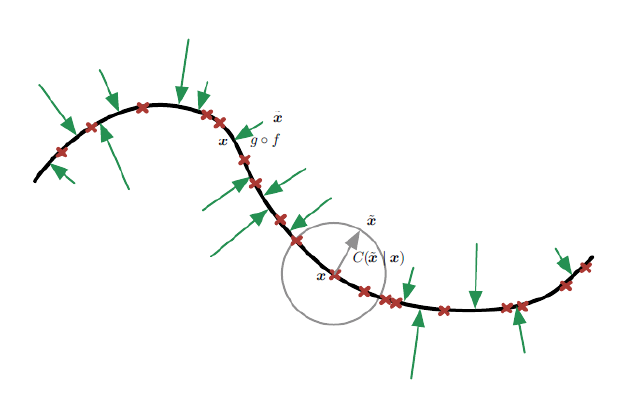
\includegraphics[width=1\textwidth]{figures/Fernandes/DAE_processo_degradacao.png}
        \end{column}
        \begin{column}{0.5\textwidth}
            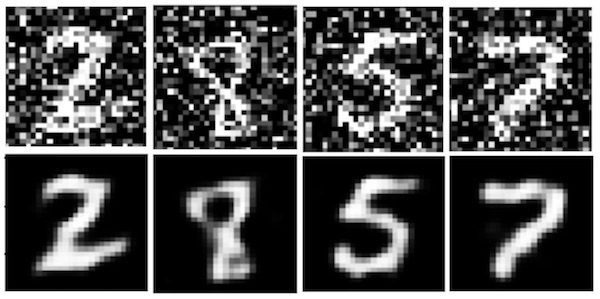
\includegraphics[width=0.8\textwidth]{figures/Fernandes/DAE_exemplo.jpg}
            % https://learnopencv.com/understanding-autoencoders-using-tensorflow-python/
            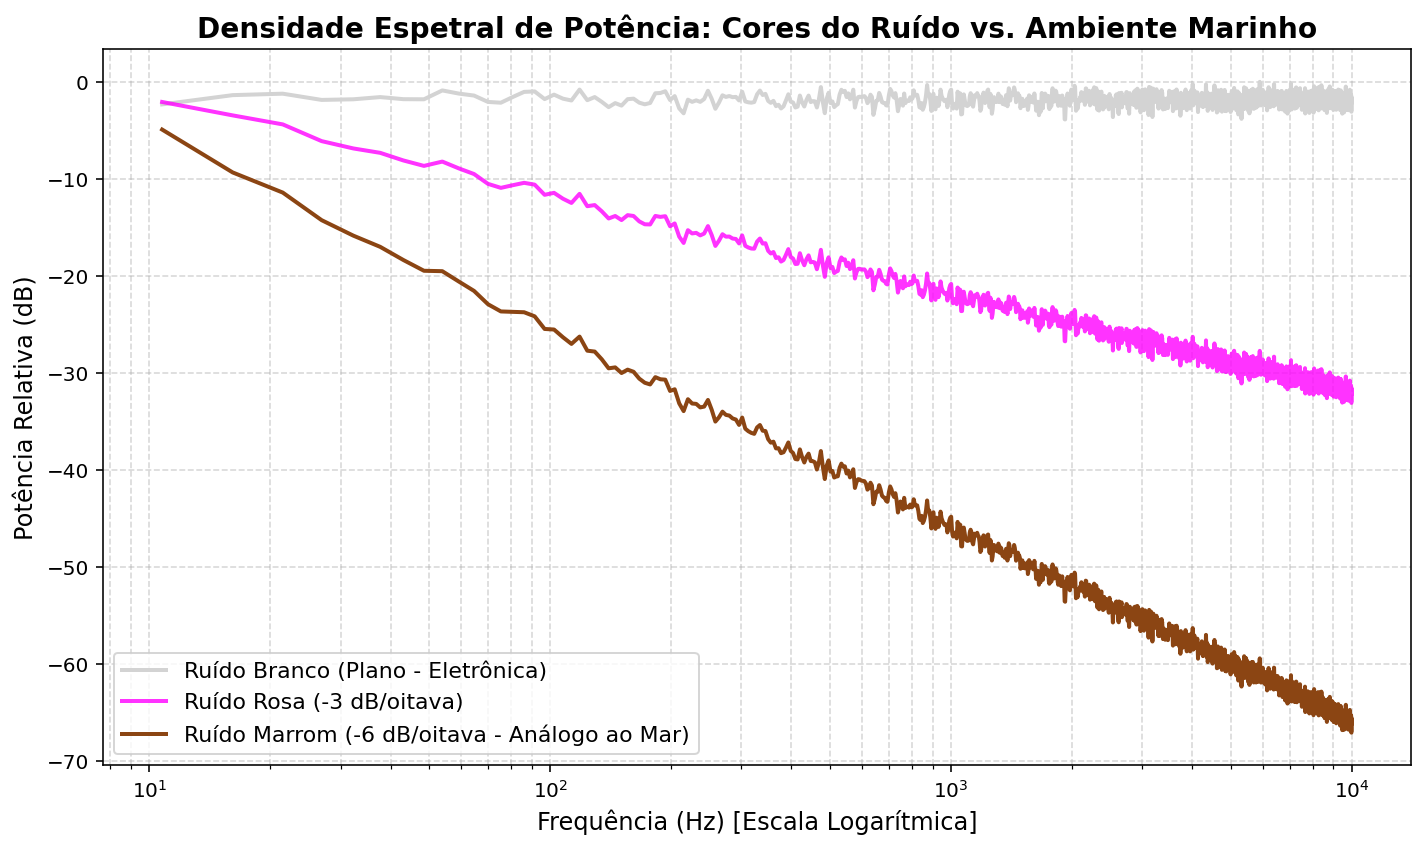
\includegraphics[width=0.8\textwidth]{figures/Fernandes/DAE_ruidos_marinho.png}
        \end{column}
    \end{columns}
\end{frame}

\begin{frame}{Denoising Autoencoders: Campo Vetorial e Score}
    \begin{block}{Score}
        Gradiente do logaritmo da densidade de probabilidade dos dados
        \vspace{5}
        \centering
        \\$\nabla_x \log p(x)$
        \vspace{5}
        \\Conhecer esse campo gradiente é uma forma de conhecer a estrutura dos dados!
    \end{block}    
    \begin{equation}
        g(f(\tilde{x})) - \tilde{x}
    \end{equation}
    Onde:
    \\$\tilde{x}$ é o sinal ruidoso
    \\$f(\tilde{x})$ é o código latente gerado pelo encoder
    \\$g(f(\tilde{x}))$ é o sinal reconstruído pelo Decoder
    \vspace{5}
    
    \\ OBS: Sob condições específicas, é equivalente a uma RBM.
    %Denoising training of a specific kind of autoencoder (sigmoidal hidden units, linear reconstruction units) using Gaussian noise and mean squared error
    %Score matching applied to RBMs yields a cost function that is identical to reconstruction error combined with a regularization term similar to the contractive penalty of the CAE
    
\end{frame}

\begin{frame}{Denoising Autoencoders: Campo Vetorial e Score}
    \begin{columns}
        \column{0.5\textwidth}
            \centering
            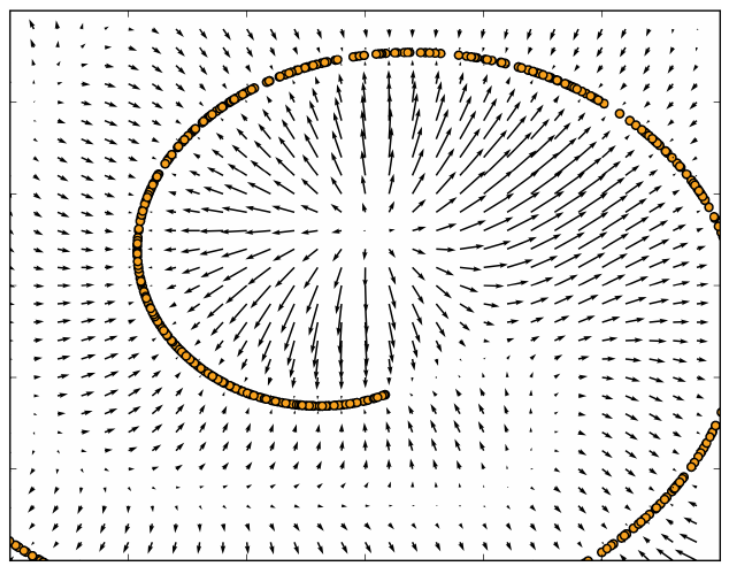
\includegraphics[width=0.95\textwidth]{figures/Fernandes/DAE_campo_vetorial_score.png}
            \vspace{-0.2cm}\\
            {\scriptsize \textit{Campo vetorial convergindo para o manifold dos dados.}}
        
        \column{0.5\textwidth}
            \small
            \begin{itemize}
                \item \textbf{Teorema \cite{alain2013}:}
                Uma arquitetura genérica estima o \textit{score}, se treinada com:
                \begin{enumerate}
                    \item Custo MSE: 
                    $\|g(f(\tilde{x})) - x\|^2$
                    \vspace{3}
                    \item Degradação Gaussiana: 
                    $\mathcal{N}(\tilde{x}; \mu=x, \Sigma=\sigma^2 I)$
                \end{enumerate}
                \vspace{0.1cm}
                \item \textbf{Interpretação:} O vetor aponta para a estrutura original (sem degradação).
            \end{itemize}
    \end{columns}
    \vspace{10}
    \centering
    Precursor de modelos gerativos que recuperam a distribuição dos dados.
\end{frame}


%------------------------------------------------

\section{Contractive Autoencoders}

\begin{frame}{Contractive Autoencoders}
    \begin{itemize}
        \item Regularização explicita em $h = f(x)$, de forma que as derivadas de $f$ devem ser menores possíveis;
        \item Norma de Frobenius da matriz Jacobiana:
    \end{itemize}
     \[
        \Omega(h) = \lambda \left\| \frac{\partial f(x)}{\partial x} \right\|_F^2
    \]
    \begin{itemize}
        \item melhor desempenho em classificadores quando esta regularização é aplicada a $f(x)$ do que a $g(f(x))$;
        \item CAE são treinados para resistir a pertubações na entrada e mapear entradas próximas para uma vizinhança menor;
        Contudo, dois pontos diferentes $x$ e $x'$ são mapeados para regiões mais distantes $f(x)$ e $f(x')$.
    \end{itemize}
\end{frame}

\begin{frame}{Contractive Autoencoders}
    \centering
    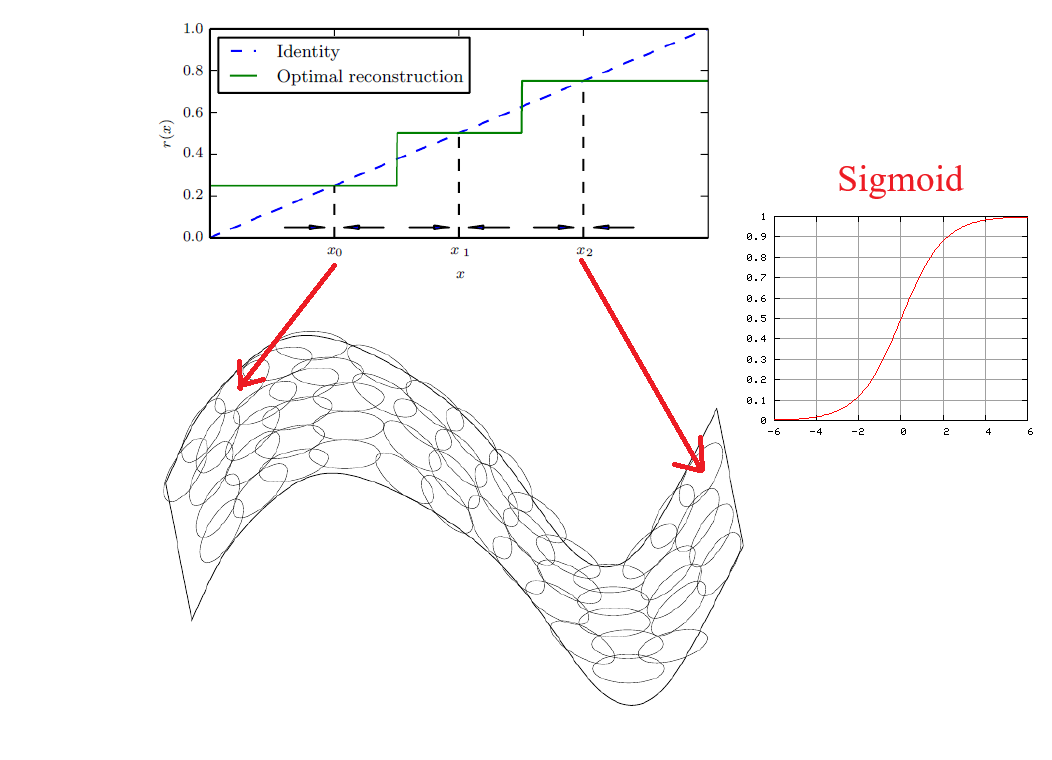
\includegraphics[width=0.75\textwidth]{figures/Fernandes/CAE.png}
\end{frame}

\begin{frame}{Contractive Autoencoders}
    \begin{block}{Treinamento dos CAE}
        \begin{itemize}
            \item Erro de reconstrução $\rightarrow$ aprender a identidade
            \item Penalidade contrativa $\rightarrow$ extração de características
        \end{itemize}
    \end{block}
    \begin{itemize}
        \item Poucas características terão derivadas significativas, estas derivadas definem o Manifold e as variáveis importantes (direções tangentes).
        \item Tendência de posicionar dados distintos em arestas do hipercubo no espaço latente, interpretando-as como um código binario. Ex: [0, 1, 1 ..., 0].
        \item Autoencoders profundos devem aplicar a Regra da Cadeia para cálculo da Matriz Jacobiana, o que seria muito pesado. Treina h1, descarta o decoder, congela a primeira camada e treina h2... $(x \rightarrow h_1 \rightarrow h_2 \rightarrow h_3...)$
        \item Previnir o erro de escala $\epsilon$  amarrando os pesos da matriz $W$,  $h = f(x)$, com a sua transposta $W^T$, para a reconstrução $g(h)$.
    \end{itemize}
\end{frame}


%------------------------------------------------
\section{Predictive Sparse Decomposition}

\begin{frame}{Predictive Sparse Decomposition}
    \begin{block}{Combinação de cracterísticas:}
        \begin{itemize}
            \item Sparse Coding $\rightarrow$ punição pelo número de ativações (L1)
            \item Parametric Autoencoders $\rightarrow$ Encoder f(x) e Decoder g(h) -- $\sigma(W_f \cdot x + b_f)$
        \end{itemize}
    \end{block}
    \[ \| x - g(h) \|^2 + \lambda |h|_1 + \gamma \| h - f(x) \|^2 \]
    \vspace{}
    \\Treinamento ocorre de forma alternada:
    \\- minimiza h, que decorre do chute inicial de f(x) + SGD
    \\- minimiza os parâmetros, backpropagation
    
\end{frame}

\begin{frame}{Predictive Sparse Decomposition: Treinamento \cite{kavukcuoglu2008}}
    \begin{itemize}
        \item A rede é iniciada com pesos e bias aleatórios;
        \item Estima-se um valor de $h$, com base nos parâmetros existentes;
        \item Utilizado o Gradiente Descendente para otimizar $h$, minimizando: 
        \[ \| x - g(h) \|^2 + \lambda |h|_1 + \gamma \| h - f(x) \|^2 \]
        \item Ajusta os parâmetros para melhor reconstrução:
        \\Decoder $g(h)$: melhor reconstrução do sinal $\rightarrow \| x - g(h) \|^2$
        \\Encoder $f(x)$: estimativa de $h$ seja mais próxima da real $\rightarrow \gamma \| h - f(x) \|^2$
        \item Após amplamente treinada, ao receber um sinal novo, a rede terá uma boa base para a inferência de $h$!
    \end{itemize}
\end{frame}

\begin{frame}{Predictive Sparse Decomposition: Emprego Real}
    \centering
    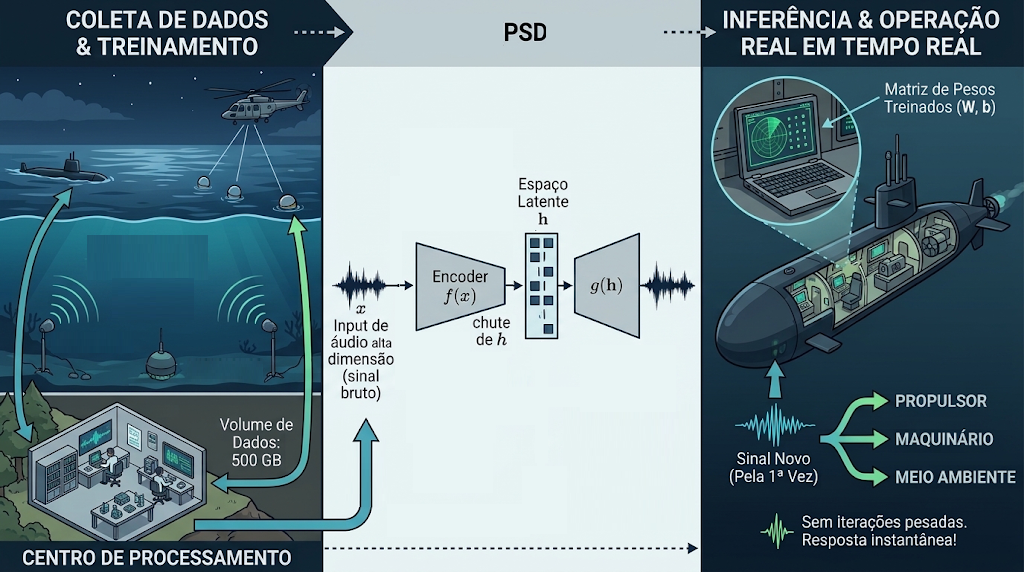
\includegraphics[width=0.85\textwidth]{figures/Fernandes/PSD_esquematico.png}
\end{frame}


%------------------------------------------------
\section{Aplicações Modernas de Autoencoders - Artigos}

\begin{frame}{Aplicações de Autoencoders}
    \begin{itemize}
        \item Redução de dimensionalidade
        \item Melhora na realização de algumas tarefas tais como Classificação, com o uso de menos memória e tempo
        \item Busca e recuperação de informações por meio de bibliotecas em espaços de baixa dimensão, por vezes binário.
    \end{itemize}
\end{frame}

\begin{frame}{Aplicações Modernas de Autoencoders - Interpretabilidade}
    Sparse Autoencoders Find Highly Interpretable Features in Language Models \cite{cunningham2024}
    \begin{itemize}
        \item \textbf{Problema:} neurônios de modelos de linguagem são \textbf{polissemânticos}, ou seja, ativam em contextos sem relação entre si. Hipótese: há mais \textit{features} do que neurônios.
        \item \textbf{O Papel do Sparse Autoencoder:} reconstrói as ativações internas do modelo com código \textbf{overcomplete} e \textbf{penalidade L1}. Cada unidade do código vira uma \textit{feature} de um ``dicionário''.
        \item \textbf{Ganhos Obtidos:}
            \\\textit{Features} \textbf{mais interpretáveis} que neurônios, PCA e ICA (avaliação automática);
            \\Remover \textit{features} permite \textbf{editar o modelo} (ex.: retirar a predição de pronomes) com menos efeitos colaterais.
    \end{itemize}
\end{frame}
 
\begin{frame}{Aplicações Modernas de Autoencoders - Interpretabilidade}
    \centering
    \vspace*{\fill}
    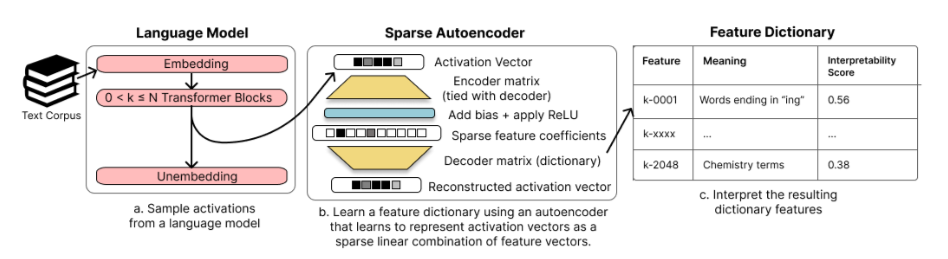
\includegraphics[width=1\textwidth]{figures/Alice/language_autoencoders.png}\\
    {\scriptsize Fonte: \cite{cunningham2024}, fig. 1.}
    \vspace*{\fill}
\end{frame}



\begin{frame}{Aplicações Modernas de Autoencoders: Tomografia}
    Improved Predictive Sparse Decomposition Method with DenseNet for Prediction of Lung Cancer \cite{mienye2020}

    \begin{itemize}
        \item \textbf{Inovação:} Substitui a restrição de esparsidade clássica da norma $L_1$ por um operador de aproximação não linear baseado na norma $L_2$.
        \item \textbf{O Papel do PSD:} Atua como um Encoder não supervisionado para extração rápida de características, gerando uma matriz esparsa a partir das imagens de TC.
        \item \textbf{Classificação:} A matriz esparsa gerada pelo PSD alimenta uma rede convolucional DenseNet de 5 camadas, que realiza o diagnóstico final.
        \item \textbf{Ganhos Obtidos:}
            \\\textbf{Redução significativa do tempo} computacional necessário para interpretar as imagens médicas.
            \\Atingiu \textbf{95\% de precisão} na detecção de câncer de pulmão, superando arquiteturas de ponta como ResNet (92\%), CNNs (88\%) e SVM (92\%)
        \end{itemize}
\end{frame}


\begin{frame}{Aplicações Modernas de Autoencoders: Acústica Sub.}
    Denoising Representation Framework for Underwater Acoustic Signal Recognition \cite{zhou2020}
    \begin{itemize}
        \item \textbf{Inovação:} Denoising Autoencoders necessitam sinais "limpos", irreais no ambiente marinho. O modelo DRR gera seus próprios alvos via correlação cruzada com o ruído ambiente e operação de \textit{dropout}.
        \item \textbf{A Arquitetura CDAE-RF:}
        \\Utiliza a estrutura completa de vários Convolutional Denoising Autoencoders (CDAE) de forma paralela.
        \\A entrada recebe espectros de correlação ($R_i$) e a saída extrai a imagem reconstruída sem ruído ($S_i$) diretamente da última camada do Decoder.
        \\A imagem limpa gerada pelo Decoder alimenta um classificador Random Forest.
        \item \textbf{Ganhos Obtidos:} Supressão de ruído superior a métodos tradicionais como STFT, HHT e MFCC.
        \\Atingiu \textbf{93,83\% de acurácia} na classificação, superando outras arquiteturas baseadas em Autoencoders.
    \end{itemize}

    
\end{frame}

\begin{frame}{Aplicações Modernas de Autoencoders: Acústica Sub.}
    \centering
    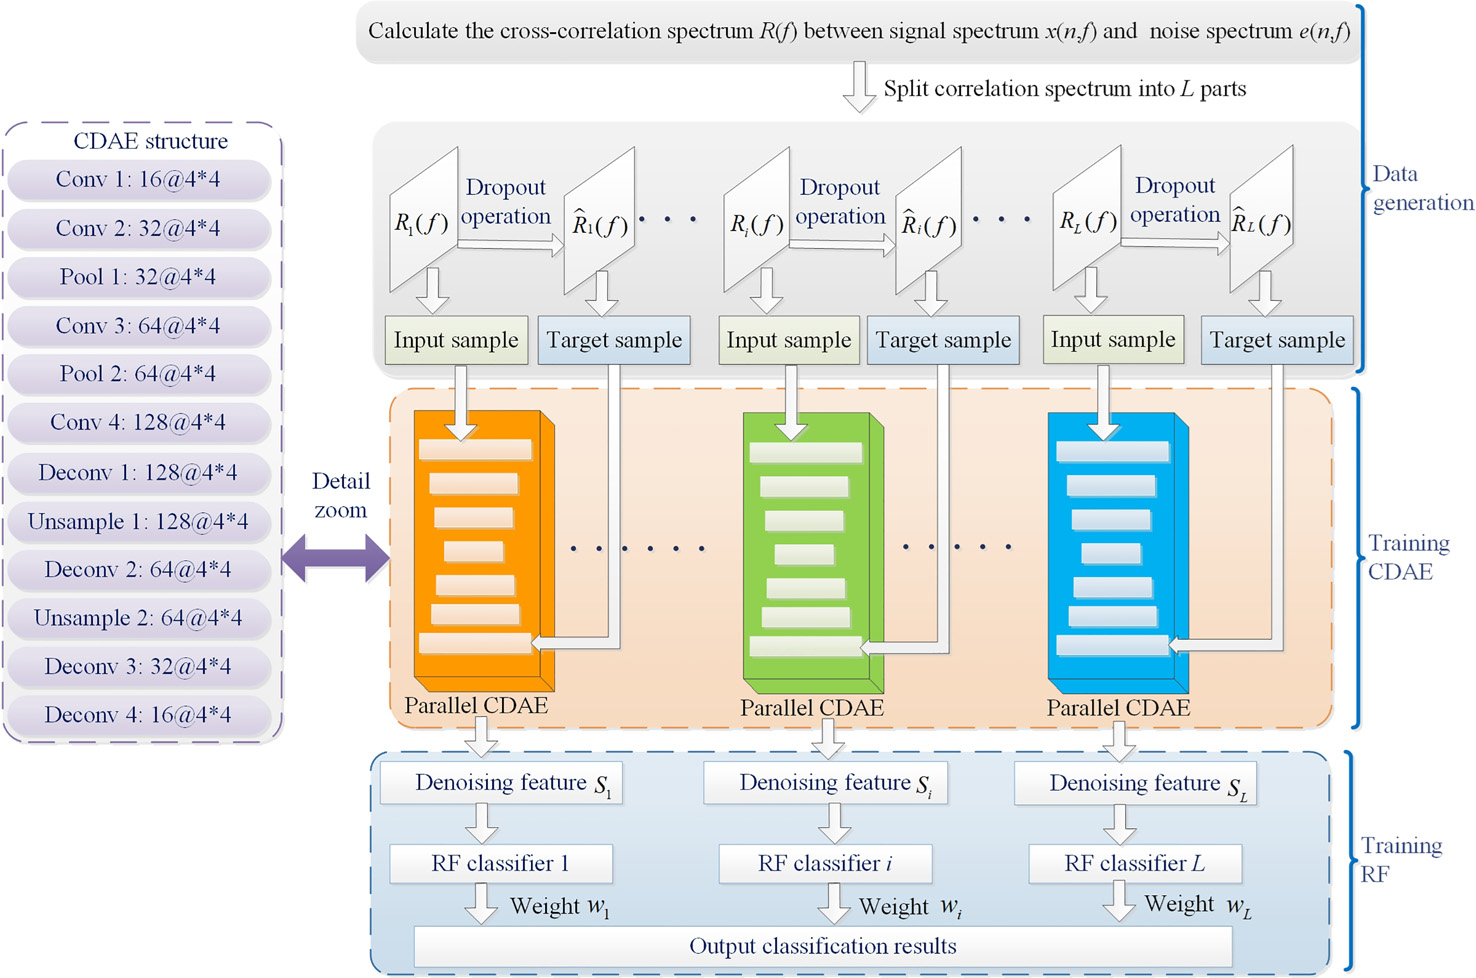
\includegraphics[width=0.7\textwidth]{figures/Fernandes/CDAE.png}    
\end{frame}
%------------------------------------------------
\section{Exemplos}

\begin{frame}{Exemplos: Emprego de DAE}
    \centering
    Comparação na reconstrução de imagens entre PCA e DAE
    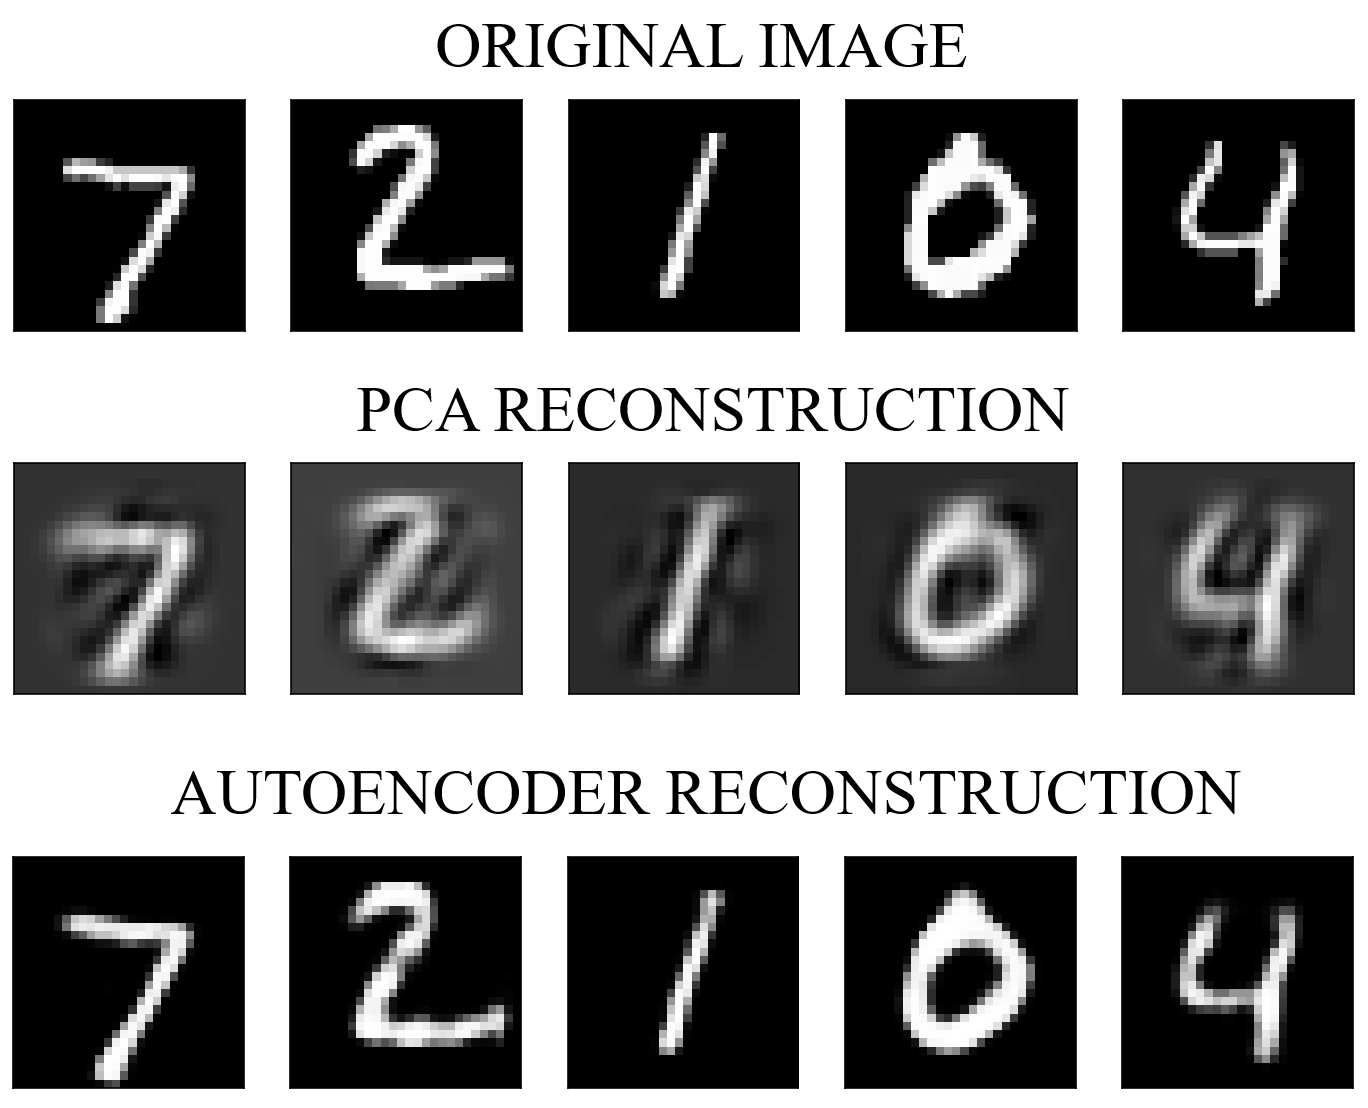
\includegraphics[width=0.45\textwidth]{figures/Fernandes/DAE_MNIST.png}
    \url{https://medium.com/@ompramod/autoencoders-explained-9196c38af6f6}
\end{frame}

\begin{frame}{Exemplos - Reconstrução da LOFAR de Embarcações \cite{lofar_book_ref}}
\begin{columns}
    \begin{column}{0.45\textwidth}
        Entrada:\\
        \texttt{Input(shape=(512,))}\vspace{0.5cm}
                
        Encoder:\\
        \texttt{Dense(128, activation='relu')}\\
        \texttt{h = Dense(32, activation='relu')}\vspace{0.5cm}
        
        Decoder:\\
        \texttt{Dense(128, activation='relu')(h)}\\
        \texttt{Dense(512, activation='sigmoid')}\vspace{0.5cm}

        Treinamento:\\
        \texttt{epochs=200}\\
        \texttt{patience=10}\\
        treinamento parou com 143 épocas.        
    \end{column}

    \begin{column}{0.50\textwidth}
        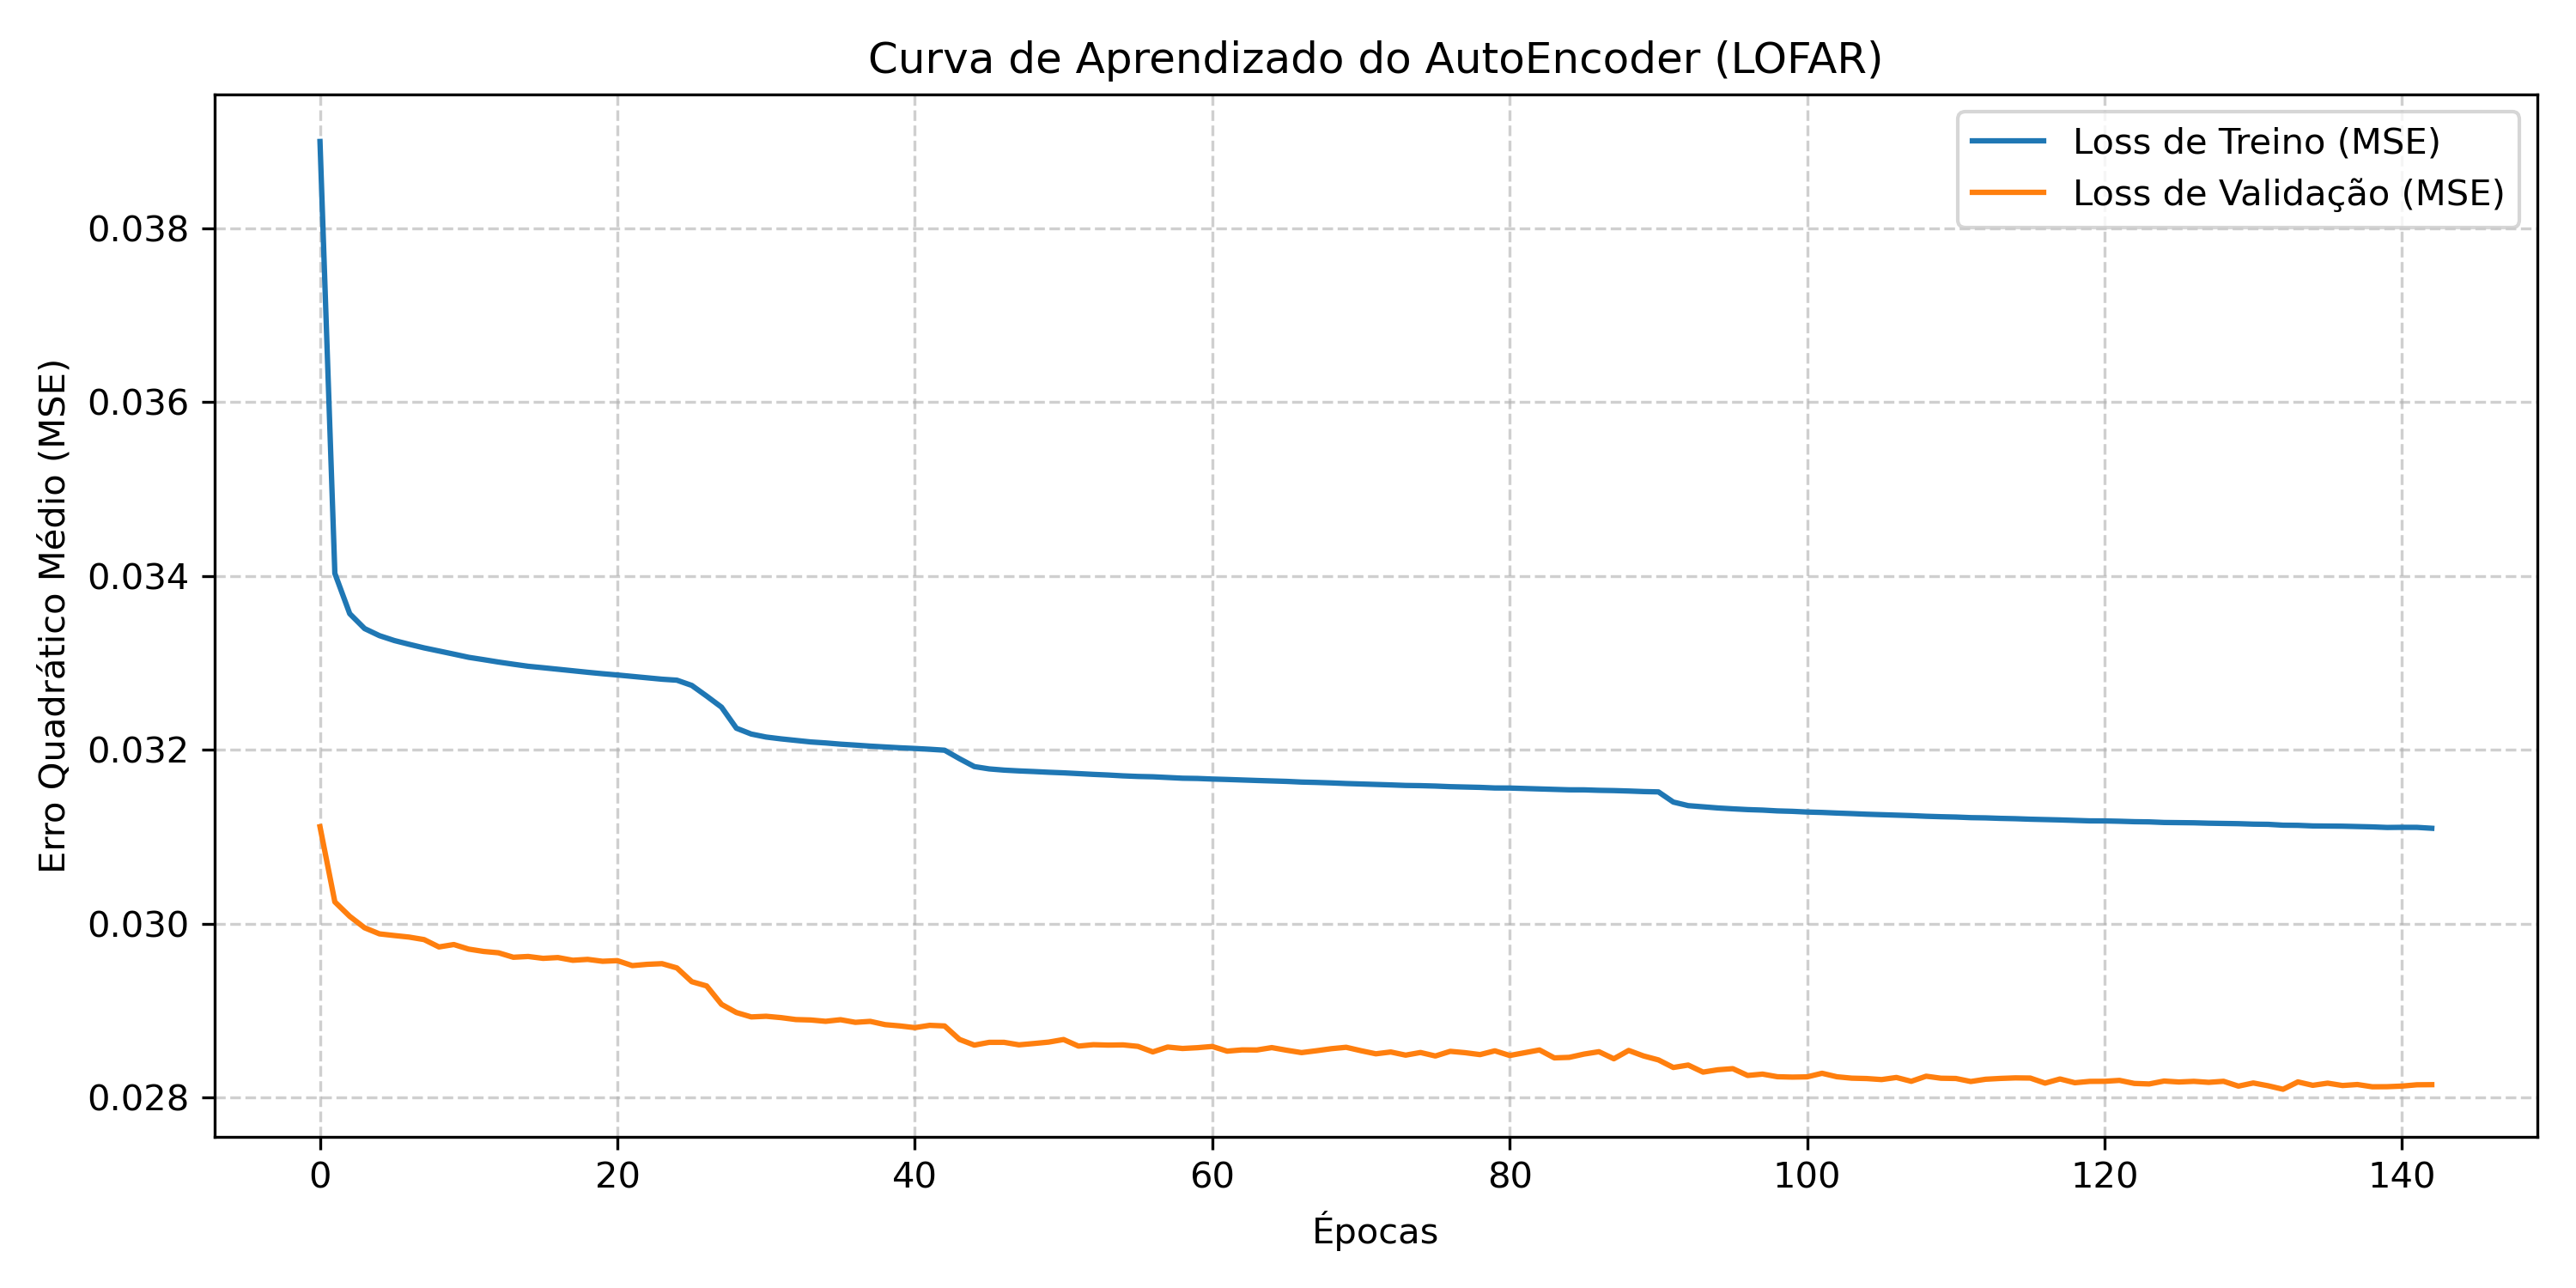
\includegraphics[width=1.0\textwidth]{figures/Fernandes/curva_aprendizado_DAE_LOFAR.png}
    \end{column}
\end{columns}

\end{frame}

\begin{frame}{Exemplos: Reconstrução da LOFAR de Embarcações}
    \centering
    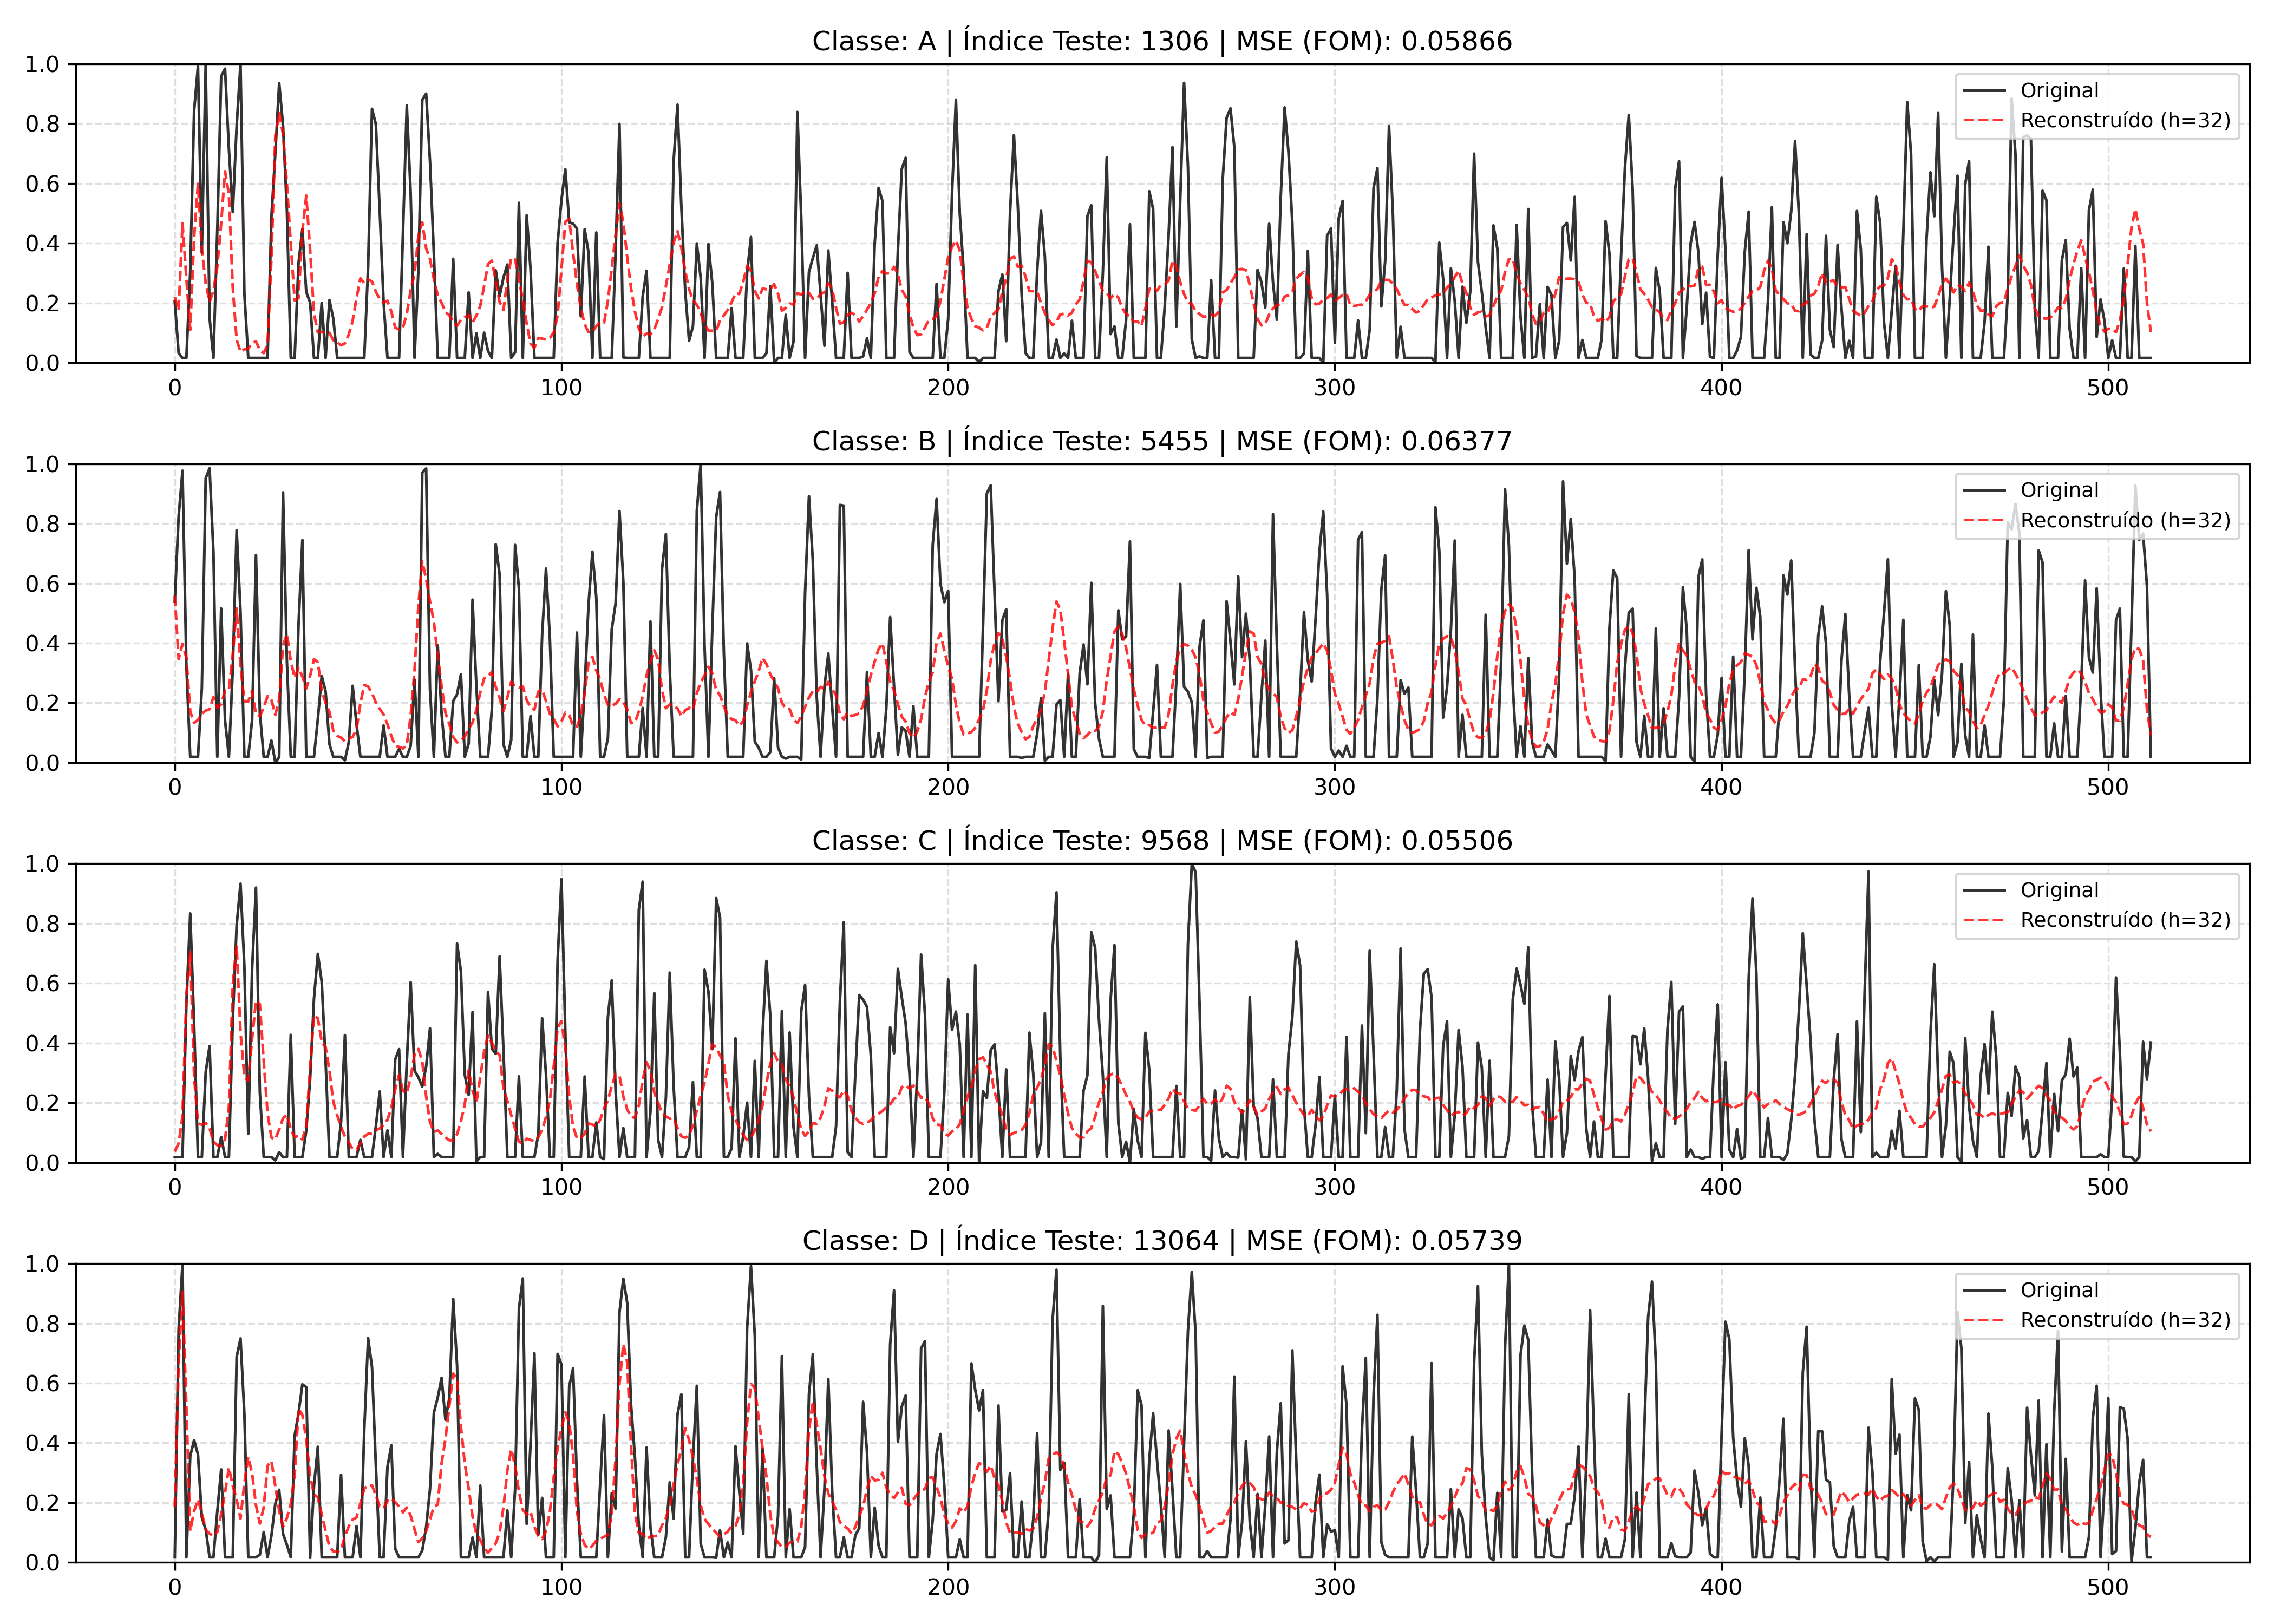
\includegraphics[width=0.65\textwidth]{figures/Fernandes/comparacao_reconstrucao.png}
\end{frame}


%\begin{frame}{Exemplos: Classificação MLP LOFAR}
%    \centering
%    Aplicada a camada latente (h) como entrada para uma rede de Classificação de Sinais de Embarcações:\\
%    \includegraphics[width=0.4\textwidth]{figures/Fernandes/xxx}
%\end{frame}

\begin{frame}{Finalidade para a pesquisa acadêmica}
    \centering
    Pré-Projeto apresentado à COPPE\\
    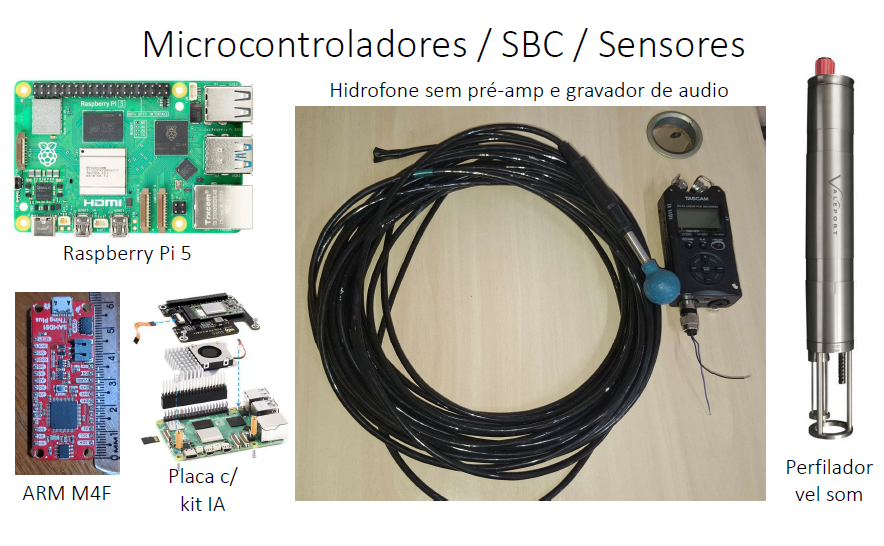
\includegraphics[width=0.75\textwidth]{figures/Fernandes/pre_projeto.png}
\end{frame}

\begin{frame}{Dúvidas}
    \centering
    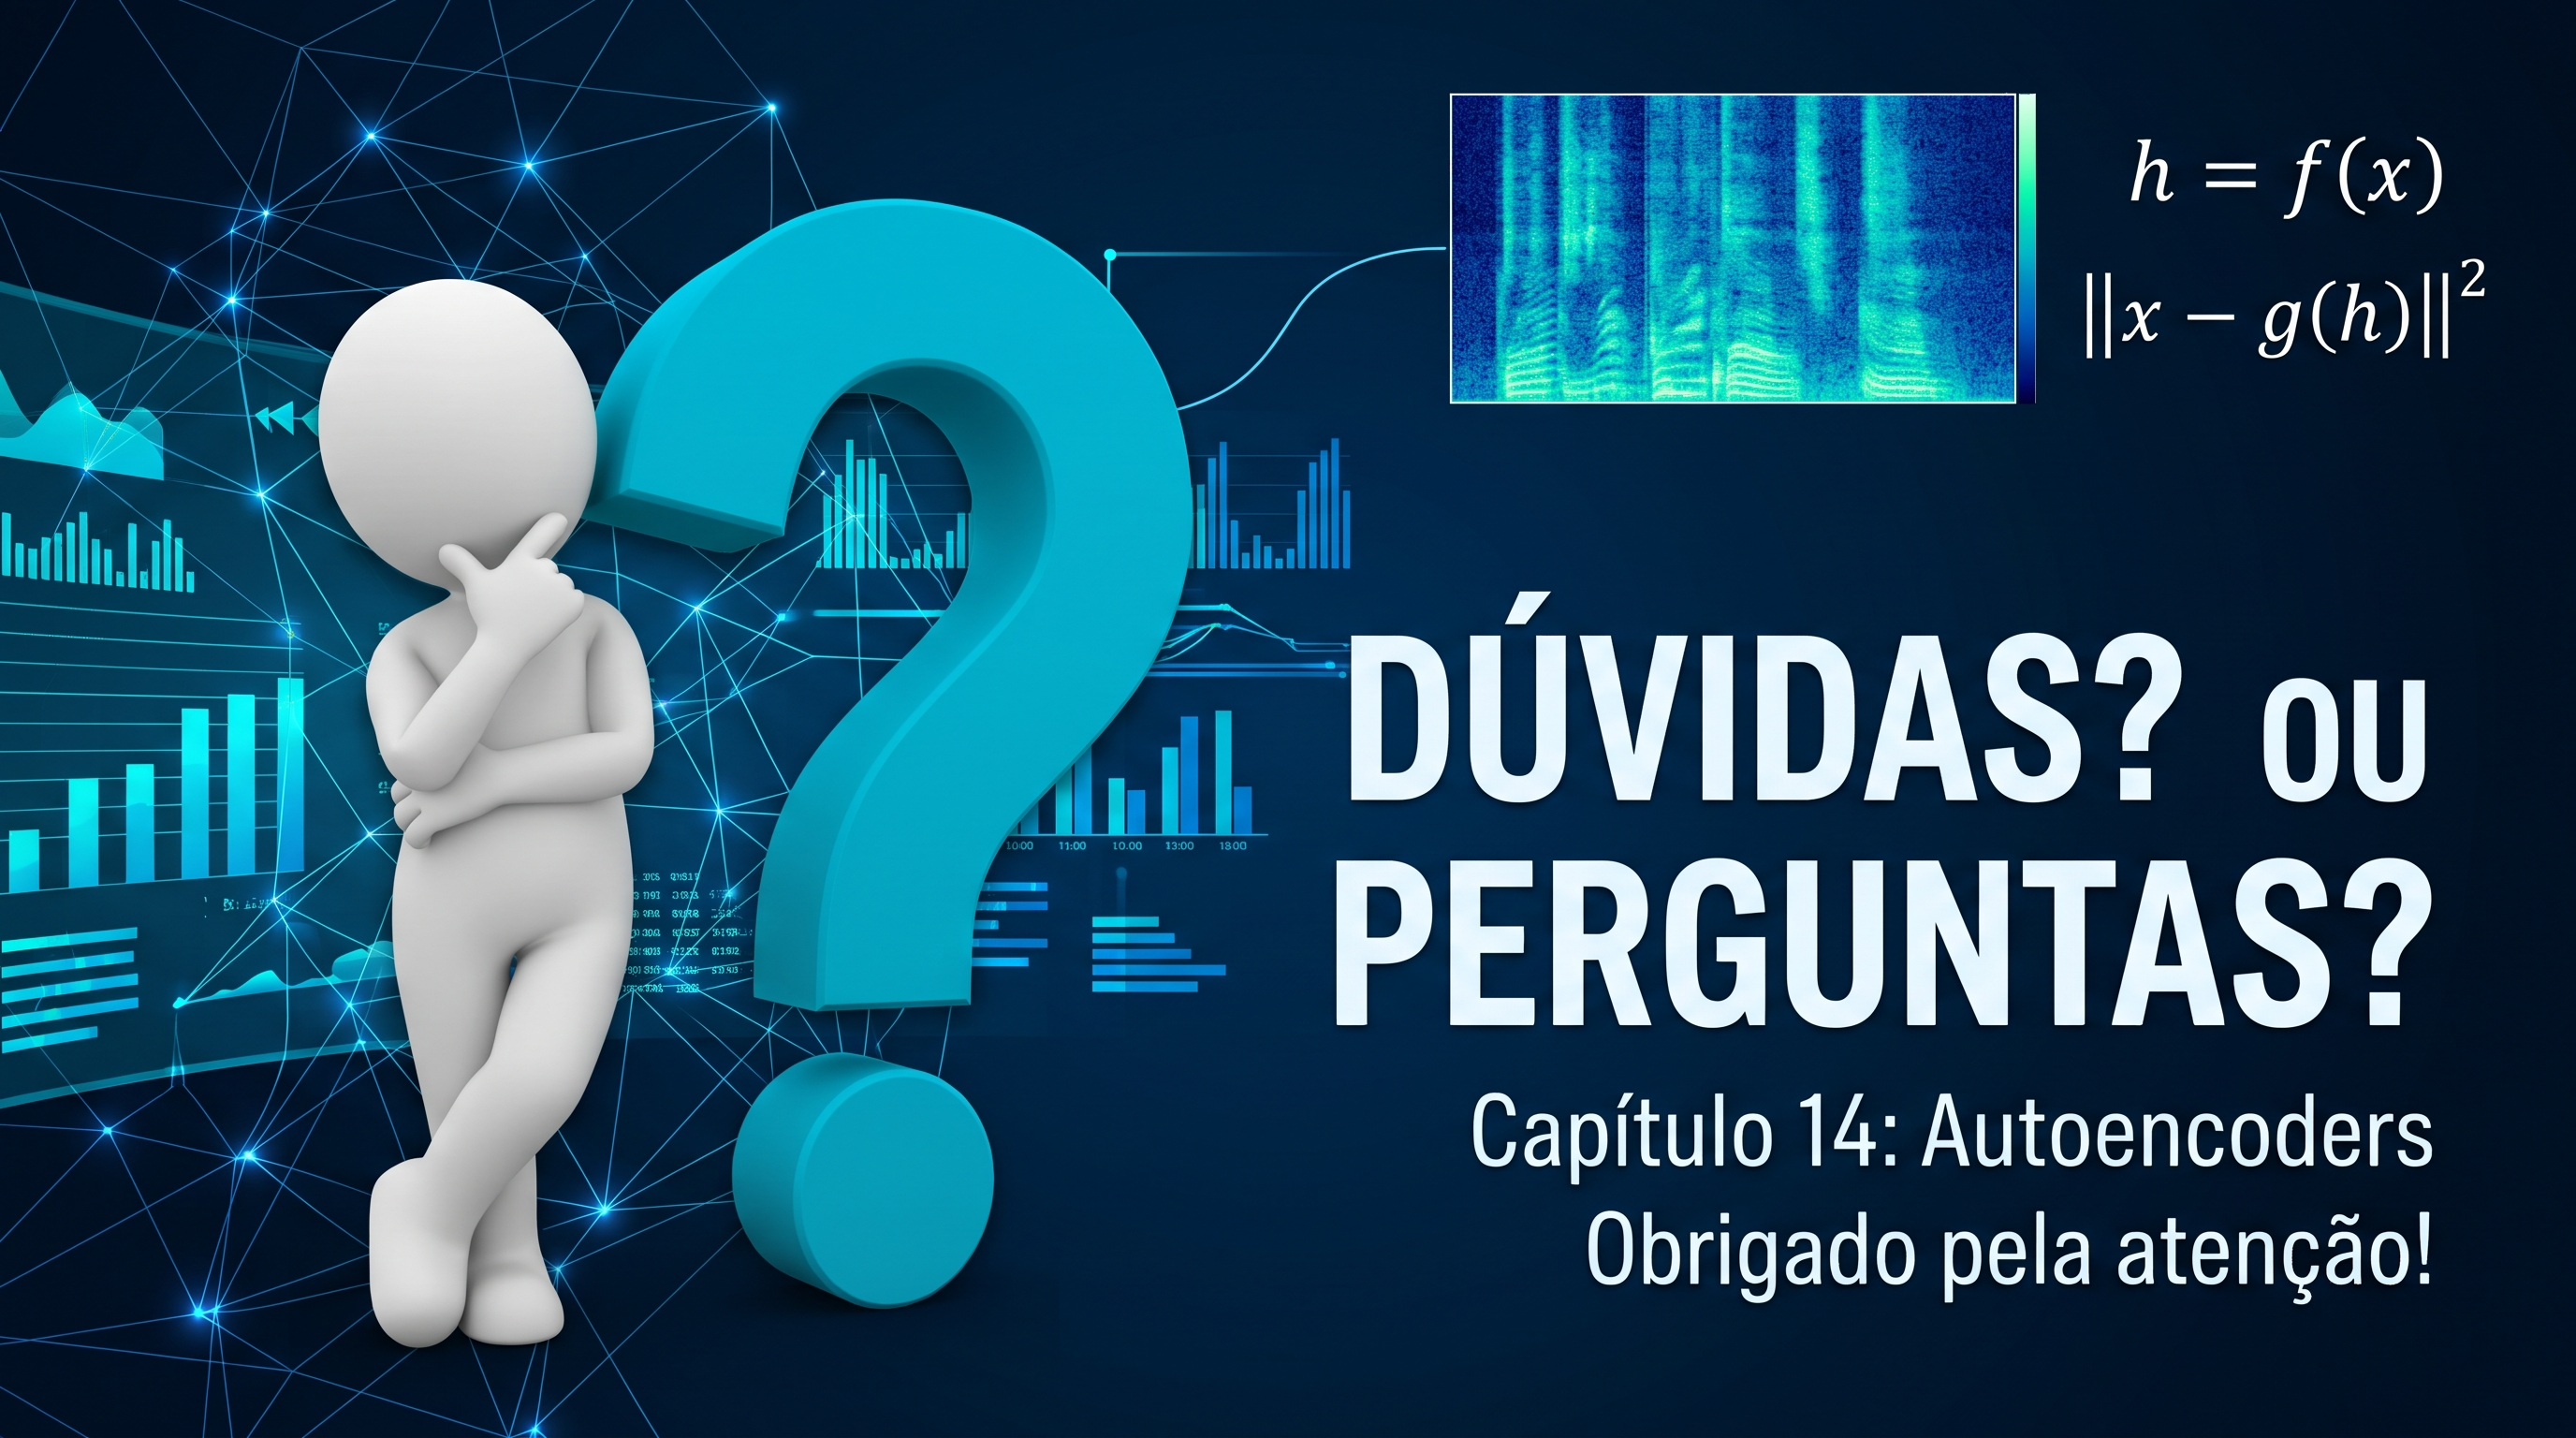
\includegraphics[width=0.85\textwidth]{figures/Fernandes/Perguntas.jpg}
\end{frame}


\begin{frame}{Informações de Contatos}
        \begin{columns}[t]
        \begin{column}{0.5\textwidth}
            \centering
            \textbf{Nome:} Alice Cipriano
            \vspace{2.0cm}

            \small
            \textbf{E-mail:} \href{mailto:alice.cipriano@lps.ufrj.br}{alice.cipriano@lps.ufrj.br}\\[0.1cm]
            \textbf{GitHub:} \href{https://github.com/alicecipriano25}{github.com/alicecipriano25}
        \end{column}
        \begin{column}{0.5\textwidth}
            \centering
            \textbf{Nome:} Leandro Fernandes
            \vspace{5}
            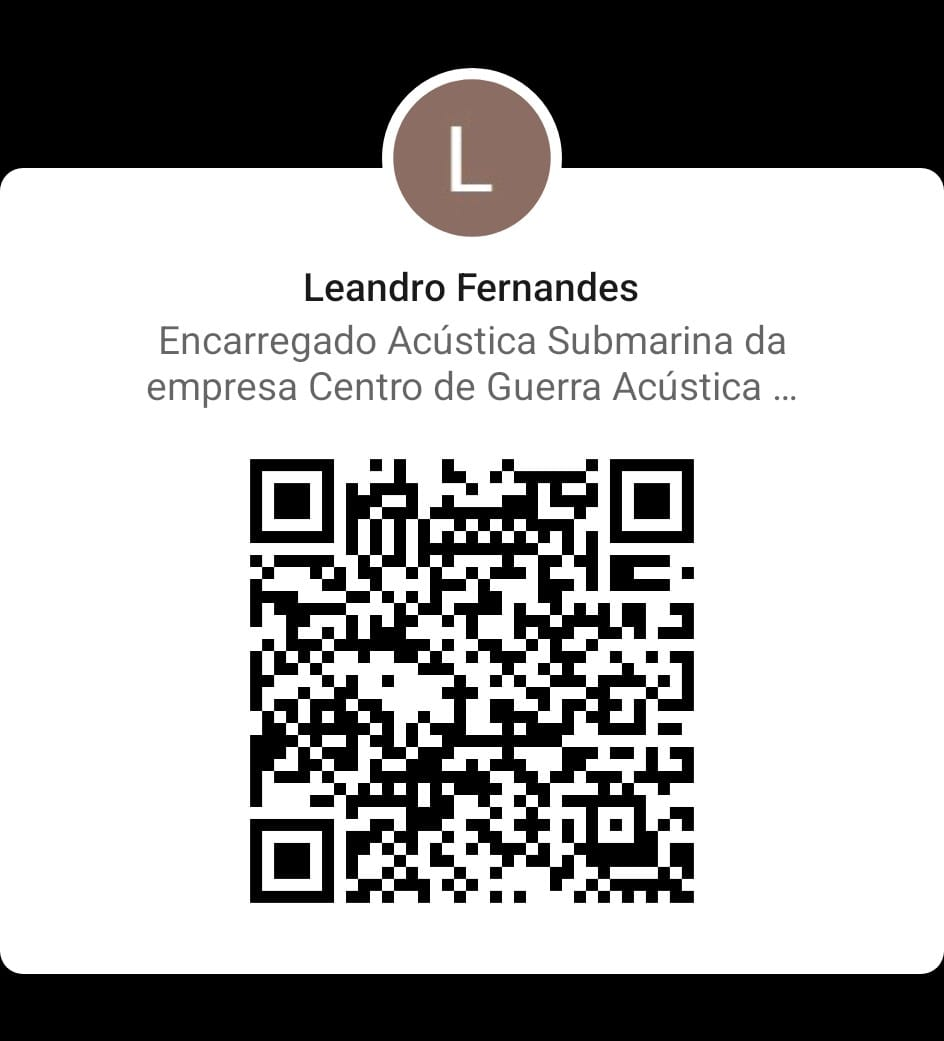
\includegraphics[width=0.8\textwidth]{figures/Fernandes/qr_linkedin.jpeg}
        \end{column}
    \end{columns}
\end{frame}

%------------------------------------------------

\begin{frame}[allowframebreaks]
\frametitle{Referências}
    \footnotesize
    \bibliographystyle{ieeetr}
    \bibliography{reference.bib}
    
\end{frame}

%------------------------------------------------


\end{document}